\documentclass[../../main.tex]{subfiles}
\newcommand{\DiagramaEscala}{0.9}
\begin{document}

\section{Raíces de Ecuaciones}

%==================================================
% INTRODUCCIÓN
%==================================================

\subsection{Introducción}

\begin{frame}{Motivación}

Desde hace años usted aprendió a usar la fórmula cuadrática:

\[
x = \frac{-b \pm \sqrt{b^2 - 4ac}}{2a}
\]

para resolver ecuaciones de la forma:

\[
f(x)=ax^2+bx+c=0
\]

\begin{itemize}
    \item Los valores calculados se llaman \textbf{raíces} de la ecuación.
    \item Representan los valores de \(x\) que hacen que
    \[
    f(x)=0.
    \]
    \item Por esta razón, también se conocen como \textbf{ceros de la función}.
\end{itemize}

\end{frame}


%--------------------------------------------------

\begin{frame}{Limitaciones de la Fórmula Cuadrática}
\begin{itemize}

    \item La fórmula cuadrática permite encontrar directamente las raíces de una ecuación de segundo grado.

    \item Sin embargo, existen muchas ecuaciones cuyas raíces no pueden determinarse mediante una expresión algebraica sencilla.

    \item Algunos ejemplos incluyen:
    \begin{itemize}
        \item funciones trascendentales,
        \item polinomios de alto grado,
        \item ecuaciones provenientes de modelos de ingeniería.
    \end{itemize}
    \item En estos casos se utilizan \textbf{métodos numéricos} para obtener aproximaciones de las raíces.

    \begin{itemize}
        \item Método de bisección.
        \item Método de falsa posición.
        \item Método de punto fijo.
        \item Método de Newton-Raphson.
        \item Método de la secante.
    \end{itemize}

\end{itemize}

\end{frame}


%==================================================
% MÉTODOS CERRADOS
%==================================================

\subsection{Métodos Cerrados}

\begin{frame}{Métodos Cerrados para Encontrar Raíces}

\begin{itemize}

    \item Se basan principalmente en el \textbf{cambio de signo} de una función alrededor de una raíz.

    \item Requieren dos valores iniciales que formen un intervalo que encierre la raíz.

    \item También se conocen como \textbf{métodos de intervalos}.

    \item Si \(f(x)\) es continua y

    \[
    f(x_l)f(x_u)<0,
    \]

    entonces existe al menos una raíz en el intervalo

    \[
    [x_l,x_u].
    \]

    \item Los métodos cerrados reducen sistemáticamente el tamaño del intervalo hasta localizar la raíz con la precisión deseada.

\end{itemize}

\end{frame}


%==================================================
% MÉTODOS GRÁFICOS
%==================================================

\subsubsection{Métodos Gráficos}

\begin{frame}{Métodos Gráficos}

\begin{itemize}

    \item Graficar \(f(x)\) permite observar aproximadamente los puntos donde la función cruza el eje \(x\).

    \item En esos puntos se cumple:

    \[
    f(x)=0.
    \]

    \item El cruce proporciona una \textbf{aproximación visual de la raíz}.

    \item Los métodos gráficos son útiles para:

    \begin{itemize}
        \item localizar aproximadamente las raíces,
        \item seleccionar intervalos iniciales,
        \item identificar raíces múltiples,
        \item detectar posibles discontinuidades.
    \end{itemize}

\end{itemize}

\end{frame}


%--------------------------------------------------
% EJEMPLO PARACAIDISTA
%--------------------------------------------------

\begin{frame}{Ejemplo 1: Método Gráfico}

\textbf{Problema:}

Determinar el coeficiente de resistencia \(c\) para que un paracaidista de masa

\[
m=68.1\,\text{kg}
\]

alcance una velocidad de

\[
v=40\,\text{m/s}
\]

después de

\[
t=10\,\text{s}.
\]

\vspace{0.3cm}

La ecuación que debe resolverse es:

\[
f(c)=
\frac{668.06}{c}
\left(
1-e^{-0.146843c}
\right)
-40.
\]

La solución buscada corresponde al valor de \(c\) para el cual

\[
f(c)=0.
\]

\end{frame}


%--------------------------------------------------

\begin{frame}{Evaluación y Gráfica}

\begin{columns}

\begin{column}{0.48\textwidth}

Se evalúa \(f(c)\) para diferentes valores:

\begin{center}
\begin{tabular}{|c|c|}
\hline
\(c\) & \(f(c)\) \\
\hline
4  & 34.190 \\
8  & 17.712 \\
12 & 6.114 \\
16 & -2.230 \\
20 & -8.368 \\
\hline
\end{tabular}
\end{center}

\begin{itemize}

    \item Se observa un cambio de signo entre

    \[
    c=12
    \quad\text{y}\quad
    c=16.
    \]

    \item Por tanto, existe una raíz en ese intervalo.

    \item Gráficamente:

    \[
    c\approx14.75.
    \]

\end{itemize}

\end{column}


\begin{column}{0.52\textwidth}

\centering

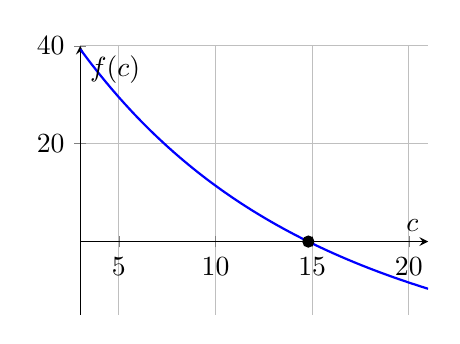
\begin{tikzpicture}

\begin{axis}[
    width=6cm,
    height=5cm,
    domain=3:21,
    samples=250,
    axis lines=middle,
    xlabel={$c$},
    ylabel={$f(c)$},
    grid=major,
    ymin=-15,
    ymax=40
]

\addplot[
    blue,
    thick,
    smooth
]
{668.06/x*(1-exp(-0.146843*x))-40};

\addplot[
    only marks,
    mark=*,
    mark size=2pt
]
coordinates {(14.8011,0)};

\end{axis}

\end{tikzpicture}

\end{column}

\end{columns}

\end{frame}


%--------------------------------------------------

\begin{frame}{Valor Práctico de los Métodos Gráficos}

Los métodos gráficos tienen una precisión limitada, pero son muy útiles como etapa preliminar.

\begin{itemize}

    \item Permiten visualizar el comportamiento general de la función.

    \item Ayudan a identificar aproximadamente la posición de las raíces.

    \item Facilitan la selección de valores iniciales para otros métodos numéricos.

    \item Permiten detectar:

    \begin{itemize}
        \item raíces múltiples,
        \item discontinuidades,
        \item regiones con varias raíces.
    \end{itemize}

\end{itemize}

Por esta razón, suelen complementar los métodos numéricos utilizados para resolver

\[
f(x)=0.
\]

\end{frame}


%--------------------------------------------------

\begin{frame}{Advertencias: Raíces Múltiples y Discontinuidades}

\begin{itemize}

    \item Una raíz de multiplicidad par puede tocar el eje \(x\) sin producir un cambio de signo.

    \item Por ejemplo:

    \[
    f(x)=(x-2)^2(x-4).
    \]

    En \(x=2\), la función tiene una raíz doble.

    \item Una discontinuidad también puede producir un cambio de signo sin que exista una raíz.

    \item Por ello, la condición

    \[
    f(x_l)f(x_u)<0
    \]

    debe aplicarse junto con la condición de que la función sea \textbf{continua} en el intervalo analizado.

\end{itemize}

\end{frame}


%--------------------------------------------------
% FUNCIÓN CON MÚLTIPLES RAÍCES
%--------------------------------------------------

\begin{frame}{Ejemplo 2: Uso de Gráficas por Computadora}

\begin{columns}

\begin{column}{0.48\textwidth}

Considere la función:

\[
f(x)=\sin(10x)+\cos(3x).
\]

\begin{itemize}

    \item Se analiza inicialmente el intervalo:

    \[
    0\leq x\leq5.
    \]

    \item La gráfica muestra la existencia de múltiples raíces.

    \item Algunas raíces están muy próximas entre sí.

    \item Por ello puede ser necesario ampliar determinadas regiones de la gráfica.

\end{itemize}

\end{column}


\begin{column}{0.52\textwidth}

\centering

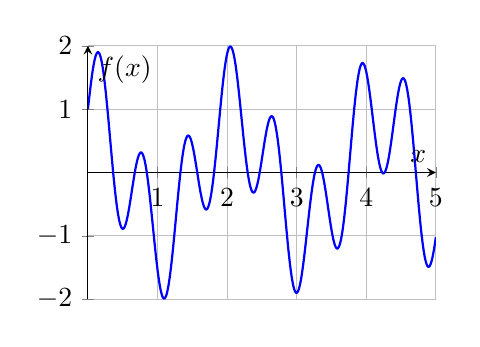
\begin{tikzpicture}

\begin{axis}[
    width=6cm,
    height=4.8cm,
    domain=0:5,
    samples=500,
    axis lines=middle,
    xlabel={$x$},
    ylabel={$f(x)$},
    xtick={0,1,...,5},
    ytick={-2,-1,0,1,2},
    grid=major,
    ymin=-2,
    ymax=2
]

\addplot[
    blue,
    thick
]
{sin(deg(10*x))+cos(deg(3*x))};

\end{axis}

\end{tikzpicture}

\end{column}

\end{columns}

\end{frame}


%--------------------------------------------------

\begin{frame}{Ampliación de una Región de la Gráfica}

Al ampliar la región cercana a

\[
x\approx4.2,
\]

se observa que existen dos raíces muy próximas.

\begin{center}

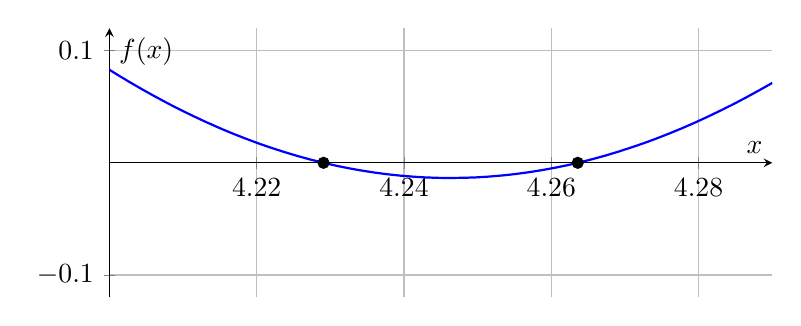
\begin{tikzpicture}

\begin{axis}[
    width=10cm,
    height=5cm,
    domain=4.20:4.29,
    samples=500,
    axis lines=middle,
    xlabel={$x$},
    ylabel={$f(x)$},
    grid=major,
    ymin=-0.12,
    ymax=0.12
]

\addplot[
    blue,
    thick
]
{sin(deg(10*x))+cos(deg(3*x))};

\addplot[
    only marks,
    mark=*,
    mark size=2pt
]
coordinates {
    (4.22907,0)
    (4.26359,0)
};

\end{axis}

\end{tikzpicture}

\end{center}

Aproximadamente:

\[
x_1\approx4.22907,
\qquad
x_2\approx4.26359.
\]

\end{frame}


%==================================================
% MÉTODO DE BISECCIÓN
%==================================================

\subsubsection{Método de Bisección}

\begin{frame}{Método de Bisección}

El método de bisección es uno de los métodos cerrados más sencillos para determinar raíces.

\begin{itemize}

    \item Se requiere que \(f(x)\) sea continua en

    \[
    [x_l,x_u].
    \]

    \item Los extremos deben cumplir:

    \[
    f(x_l)f(x_u)<0.
    \]

    \item Esta condición garantiza que existe al menos una raíz dentro del intervalo.

    \item En cada iteración el intervalo se divide en dos partes iguales.

    \item El intervalo que contiene la raíz se conserva para la siguiente iteración.

\end{itemize}

También se conoce como:

\begin{itemize}
    \item método de corte binario,
    \item método de partición de intervalos.
\end{itemize}

\end{frame}


%--------------------------------------------------

\begin{frame}{Pasos del Método de Bisección}

\begin{enumerate}

    \item Seleccionar \(x_l\) y \(x_u\) tales que

    \[
    f(x_l)f(x_u)<0.
    \]

    \item Calcular el punto medio:

    \[
    x_r=
    \frac{x_l+x_u}{2}.
    \]

    \item Evaluar

    \[
    f(x_l)f(x_r).
    \]

    \begin{itemize}

        \item Si

        \[
        f(x_l)f(x_r)<0,
        \]

        entonces:

        \[
        x_u=x_r.
        \]

        \item Si

        \[
        f(x_l)f(x_r)>0,
        \]

        entonces:

        \[
        x_l=x_r.
        \]

        \item Si

        \[
        f(x_r)=0,
        \]

        se ha encontrado la raíz exactamente.

    \end{itemize}

    \item Repetir el procedimiento hasta alcanzar la precisión deseada.

\end{enumerate}

\end{frame}


%--------------------------------------------------

\begin{frame}{Representación Gráfica del Método de Bisección}

\centering

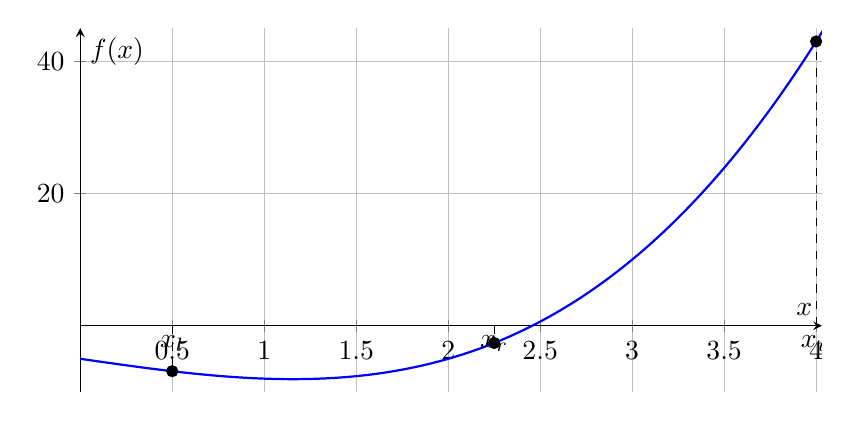
\begin{tikzpicture}

\begin{axis}[
    width=11cm,
    height=6.2cm,
    domain=0:4.2,
    samples=250,
    axis lines=middle,
    xlabel={$x$},
    ylabel={$f(x)$},
    ymin=-10,
    ymax=45,
    grid=major
]

% Función
\addplot[
    blue,
    thick
]
{x^3-4*x-5};

% xl
\addplot[
    only marks,
    mark=*,
    mark size=2pt
]
coordinates {(0.5,-6.875)};

\node[
    below
]
at (axis cs:0.5,0)
{$x_l$};

% xu
\addplot[
    only marks,
    mark=*,
    mark size=2pt
]
coordinates {(4,43)};

\node[
    below
]
at (axis cs:4,0)
{$x_u$};

% xr
\addplot[
    only marks,
    mark=*,
    mark size=2pt
]
coordinates {(2.25,-2.609375)};

\node[
    below
]
at (axis cs:2.25,0)
{$x_r$};

% Líneas
\draw[dashed]
(axis cs:0.5,0)
--
(axis cs:0.5,-6.875);

\draw[dashed]
(axis cs:4,0)
--
(axis cs:4,43);

\draw[dashed]
(axis cs:2.25,0)
--
(axis cs:2.25,-2.609375);

\end{axis}

\end{tikzpicture}

\end{frame}


%==================================================
% EJEMPLO BISECCIÓN
%==================================================

\begin{frame}{Ejemplo 3: Método de Bisección}

Encontrar mediante bisección la raíz de

\[
f(c)=
\frac{668.06}{c}
\left(
1-e^{-0.146843c}
\right)
-40.
\]

Del análisis gráfico se obtuvo:

\[
c_l=12,
\qquad
c_u=16.
\]

Además:

\[
f(12)=6.114>0,
\]

\[
f(16)=-2.230<0.
\]

Por tanto:

\[
f(12)f(16)<0,
\]

y existe una raíz en

\[
[12,16].
\]

\end{frame}


%--------------------------------------------------

\begin{frame}{Método de Bisección: Iteración 1}

El primer punto medio es:

\[
c_r=
\frac{c_l+c_u}{2}.
\]

Sustituyendo:

\[
c_r=
\frac{12+16}{2}
=14.
\]

Evaluando:

\[
f(14)\approx1.611.
\]

Como:

\[
f(12)f(14)
=
(6.114)(1.611)
>0,
\]

la raíz no se encuentra entre \(12\) y \(14\).

Por tanto, el nuevo intervalo es:

\[
[14,16].
\]

\end{frame}


%--------------------------------------------------

\begin{frame}{Error Verdadero: Iteración 1}

Para fines didácticos conocemos que la raíz verdadera es aproximadamente:

\[
c^{*}=14.8011.
\]

El error relativo porcentual verdadero es:

\[
\epsilon_t
=
\left|
\frac{c^{*}-c_r}{c^{*}}
\right|
100\%.
\]

Para

\[
c_r=14,
\]

se obtiene:

\[
\epsilon_t
=
\left|
\frac{14.8011-14}{14.8011}
\right|
100\%.
\]

Por tanto:

\[
\boxed{
\epsilon_t\approx5.41\%
}
\]

\end{frame}


%--------------------------------------------------

\begin{frame}{Método de Bisección: Iteración 2}

El nuevo intervalo es:

\[
[14,16].
\]

Calculamos:

\[
c_r=
\frac{14+16}{2}
=15.
\]

Evaluamos:

\[
f(14)\approx1.611,
\]

\[
f(15)\approx-0.384.
\]

Por tanto:

\[
f(14)f(15)<0.
\]

La raíz se encuentra entre:

\[
14<c<15.
\]

El nuevo intervalo será:

\[
[14,15].
\]

\end{frame}


%--------------------------------------------------

\begin{frame}{Error Verdadero: Iteración 2}

La aproximación obtenida es:

\[
c_r=15.
\]

El error verdadero es:

\[
\epsilon_t
=
\left|
\frac{14.8011-15}{14.8011}
\right|
100\%.
\]

Por tanto:

\[
\boxed{
\epsilon_t\approx1.34\%
}
\]

\end{frame}


%--------------------------------------------------

\begin{frame}{Método de Bisección: Iteración 3}

El nuevo intervalo es:

\[
[14,15].
\]

El punto medio es:

\[
c_r=
\frac{14+15}{2}
=14.5.
\]

Evaluando:

\[
f(14.5)>0.
\]

Por tanto, la raíz se encuentra entre:

\[
14.5<c<15.
\]

El nuevo intervalo será:

\[
[14.5,15].
\]

\end{frame}


%--------------------------------------------------

\begin{frame}{Error Verdadero: Iteración 3}

Para

\[
c_r=14.5,
\]

el error relativo verdadero es:

\[
\epsilon_t
=
\left|
\frac{14.8011-14.5}{14.8011}
\right|
100\%.
\]

Por tanto:

\[
\boxed{
\epsilon_t\approx2.03\%
}
\]

Observe que el error verdadero aumentó con respecto a la iteración anterior.

Esto muestra que:

\[
\boxed{
\text{el error verdadero no necesariamente disminuye
monótonamente en cada iteración}
}
\]

\end{frame}


%--------------------------------------------------

\begin{frame}{Comportamiento del Método de Bisección}

\begin{itemize}

    \item En cada iteración el intervalo que contiene la raíz se reduce a la mitad.

    \item Por tanto, disminuye sistemáticamente la incertidumbre sobre la posición de la raíz.

    \item Sin embargo, la aproximación del punto medio puede acercarse o alejarse temporalmente de la raíz verdadera.

    \item Por ello, el error verdadero

    \[
    \epsilon_t
    \]

    no necesariamente disminuye de manera monótona.

    \item La convergencia se garantiza porque el intervalo que contiene la raíz se hace progresivamente más pequeño.

\end{itemize}

\end{frame}


%==================================================
% ERRORES
%==================================================

\begin{frame}{Criterios de Paro y Estimación de Errores}

En aplicaciones reales normalmente no conocemos la raíz verdadera.

Por esta razón:

\begin{itemize}

    \item El error verdadero

    \[
    \epsilon_t
    \]

    no puede utilizarse directamente como criterio de paro.

    \item Se utiliza el \textbf{error relativo porcentual aproximado}:

    \[
    \epsilon_a.
    \]

    \item Este error compara dos aproximaciones consecutivas de la raíz.

\end{itemize}

\end{frame}


%--------------------------------------------------

\begin{frame}{Cálculo del Error Aproximado}

El error relativo porcentual aproximado se calcula mediante:

\[
\boxed{
\epsilon_a
=
\left|
\frac{
x_r^{\text{nuevo}}
-
x_r^{\text{anterior}}
}{
x_r^{\text{nuevo}}
}
\right|
\times100\%
}
\]

donde:

\begin{itemize}

    \item \(x_r^{\text{nuevo}}\) es la aproximación de la iteración actual.

    \item \(x_r^{\text{anterior}}\) es la aproximación obtenida en la iteración anterior.

    \item El valor absoluto permite considerar únicamente la magnitud del cambio.

\end{itemize}

\end{frame}


%--------------------------------------------------

\begin{frame}{Criterio de Paro}

Se establece previamente un error máximo permitido:

\[
\epsilon_s.
\]

El proceso iterativo se detiene cuando:

\[
\boxed{
\epsilon_a<\epsilon_s
}
\]

Por ejemplo, si se desea:

\[
\epsilon_s=0.5\%,
\]

se continúan realizando iteraciones hasta obtener:

\[
\epsilon_a<0.5\%.
\]

Este criterio permite aplicar el método sin conocer la raíz verdadera.

\end{frame}


%==================================================
% EJEMPLO ERROR
%==================================================

\begin{frame}{Ejemplo 4: Estimación del Error}

Continuaremos el ejemplo anterior hasta alcanzar:

\[
\epsilon_s=0.5\%.
\]

Las dos primeras aproximaciones fueron:

\[
c_r^{(1)}=14,
\]

\[
c_r^{(2)}=15.
\]

El primer error aproximado que puede calcularse es:

\[
\epsilon_a
=
\left|
\frac{15-14}{15}
\right|
100\%.
\]

Por tanto:

\[
\boxed{
\epsilon_a=6.667\%
}
\]

\end{frame}


%--------------------------------------------------

\begin{frame}{Iteraciones 3 y 4}

\textbf{Iteración 3}

\[
c_l=14,
\qquad
c_u=15
\]

\[
c_r=
\frac{14+15}{2}
=14.5
\]

\[
\epsilon_a
=
\left|
\frac{14.5-15}{14.5}
\right|
100
=
3.448\%.
\]

\vspace{0.3cm}

\textbf{Iteración 4}

\[
c_l=14.5,
\qquad
c_u=15
\]

\[
c_r=
14.75
\]

\[
\epsilon_a
=
\left|
\frac{14.75-14.5}{14.75}
\right|
100
=
1.695\%.
\]

\end{frame}


%--------------------------------------------------

\begin{frame}{Iteraciones 5 y 6}

\textbf{Iteración 5}

\[
c_r=
\frac{14.75+15}{2}
=
14.875
\]

\[
\epsilon_a
=
\left|
\frac{14.875-14.75}{14.875}
\right|
100
=
0.840\%.
\]

\vspace{0.3cm}

\textbf{Iteración 6}

\[
c_r=
\frac{14.75+14.875}{2}
=
14.8125
\]

\[
\epsilon_a
=
\left|
\frac{14.8125-14.875}{14.8125}
\right|
100
=
0.422\%.
\]

Como:

\[
0.422\%<0.5\%,
\]

el proceso se detiene.

\end{frame}


%--------------------------------------------------

\begin{frame}{Resumen del Ejemplo}

\centering

\small

\begin{tabular}{|c|c|c|c|c|c|}
\hline
Iter. &
\(c_l\) &
\(c_u\) &
\(c_r\) &
\(\epsilon_a(\%)\) &
\(\epsilon_t(\%)\)
\\
\hline
1 & 12    & 16     & 14      & --    & 5.413 \\
2 & 14    & 16     & 15      & 6.667 & 1.344 \\
3 & 14    & 15     & 14.5    & 3.448 & 2.035 \\
4 & 14.5  & 15     & 14.75   & 1.695 & 0.345 \\
5 & 14.75 & 15     & 14.875  & 0.840 & 0.499 \\
6 & 14.75 & 14.875 & 14.8125 & 0.422 & 0.077 \\
\hline
\end{tabular}

\vspace{0.5cm}

El cálculo se detiene en la iteración 6 porque:

\[
\epsilon_a=0.422\%<0.5\%.
\]

La aproximación obtenida es:

\[
\boxed{
c\approx14.8125
}
\]

\end{frame}


%--------------------------------------------------

\begin{frame}{Errores vs. Iteraciones}

\centering

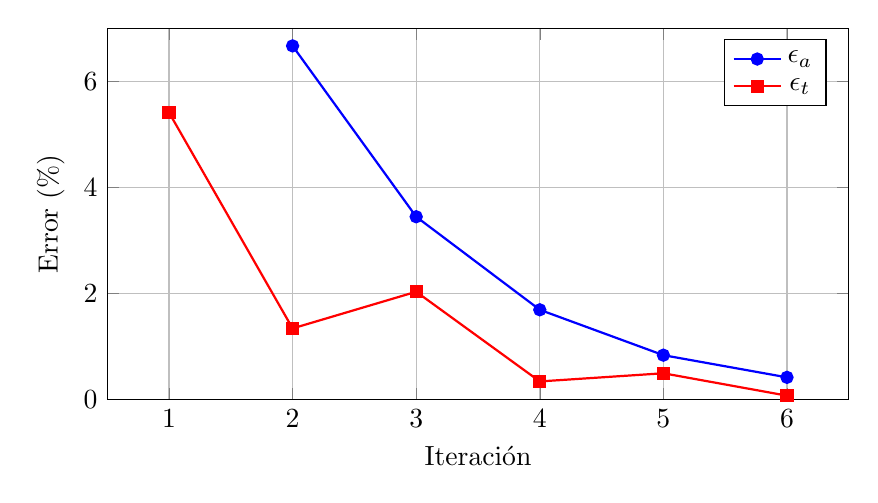
\begin{tikzpicture}

\begin{axis}[
    width=11cm,
    height=6.3cm,
    xlabel={Iteración},
    ylabel={Error (\%)},
    xtick={1,2,3,4,5,6},
    legend pos=north east,
    grid=major,
    ymin=0,
    ymax=7
]

\addplot[
    mark=*,
    blue,
    thick
]
coordinates {
    (2,6.667)
    (3,3.448)
    (4,1.695)
    (5,0.840)
    (6,0.422)
};

\addlegendentry{$\epsilon_a$}

\addplot[
    mark=square*,
    red,
    thick
]
coordinates {
    (1,5.413)
    (2,1.344)
    (3,2.035)
    (4,0.345)
    (5,0.499)
    (6,0.077)
};

\addlegendentry{$\epsilon_t$}

\end{axis}

\end{tikzpicture}

\end{frame}


%==================================================
% COTA DEL ERROR
%==================================================

\begin{frame}{Cota del Error en Bisección}

Una propiedad fundamental del método de bisección es que el intervalo que contiene la raíz se reduce a la mitad en cada iteración.

Si el intervalo actual es:

\[
[x_l,x_u],
\]

el punto medio es:

\[
x_r=
\frac{x_l+x_u}{2}.
\]

La distancia máxima entre el punto medio y cualquier punto del intervalo es:

\[
\boxed{
E_{\max}
=
\frac{x_u-x_l}{2}
}
\]

Por tanto, la raíz se encuentra dentro de:

\[
x_r
\pm
\frac{x_u-x_l}{2}.
\]

\end{frame}


%--------------------------------------------------

\begin{frame}{Error Aproximado y Cota del Error}

Es importante distinguir dos conceptos.

\textbf{Error relativo aproximado:}

\[
\epsilon_a
=
\left|
\frac{
x_r^{\text{nuevo}}
-
x_r^{\text{anterior}}
}{
x_r^{\text{nuevo}}
}
\right|
100\%.
\]

Este valor mide el cambio entre dos aproximaciones consecutivas.

\vspace{0.3cm}

\textbf{Cota del error absoluto de bisección:}

\[
E_{\max}
=
\frac{x_u-x_l}{2}.
\]

Esta última expresión proporciona una cota asociada al tamaño del intervalo que contiene la raíz.

\end{frame}


%--------------------------------------------------

\begin{frame}{Convergencia del Método de Bisección}

Si:

\begin{enumerate}

    \item \(f(x)\) es continua en

    \[
    [x_l,x_u],
    \]

    \item y se cumple

    \[
    f(x_l)f(x_u)<0,
    \]

\end{enumerate}

entonces el método mantiene al menos una raíz encerrada dentro del intervalo.

Además:

\[
\Delta x_n
=
\frac{\Delta x_0}{2^n}.
\]

Por tanto:

\[
\Delta x_n\rightarrow0
\qquad
\text{cuando}
\qquad
n\rightarrow\infty.
\]

Así, las aproximaciones convergen hacia una raíz contenida en el intervalo inicial.

\end{frame}


%==================================================
% ERROR ALTERNATIVO
%==================================================

\begin{frame}{Expresión del Error Relativo para Bisección}

Como dos puntos medios consecutivos difieren en la mitad del intervalo anterior, puede escribirse:

\[
\left|
x_r^{\text{nuevo}}
-
x_r^{\text{anterior}}
\right|
=
\frac{x_u-x_l}{2}.
\]

Además:

\[
x_r^{\text{nuevo}}
=
\frac{x_u+x_l}{2}.
\]

Por tanto:

\[
\epsilon_a
=
\left|
\frac{x_u-x_l}{x_u+x_l}
\right|
100\%.
\]

Esta expresión puede utilizarse cuando \(x_u+x_l\neq0\).

\end{frame}


%==================================================
% NÚMERO DE ITERACIONES
%==================================================

\begin{frame}{Número de Iteraciones Requeridas}

Sea el intervalo inicial:

\[
\Delta x_0
=
x_u^{(0)}
-
x_l^{(0)}.
\]

Después de \(n\) divisiones:

\[
\Delta x_n
=
\frac{\Delta x_0}{2^n}.
\]

Si se desea que el tamaño del intervalo sea menor o igual que un valor especificado:

\[
\Delta x_n
\leq
E_d,
\]

entonces:

\[
\frac{\Delta x_0}{2^n}
\leq
E_d.
\]

Despejando:

\[
\boxed{
n
\geq
\log_2
\left(
\frac{\Delta x_0}{E_d}
\right)
}
\]

\end{frame}


%--------------------------------------------------

\begin{frame}{Ejemplo: Número de Iteraciones}

Suponga:

\[
\Delta x_0=4
\]

y se desea:

\[
E_d=0.0625.
\]

Entonces:

\[
n
\geq
\log_2
\left(
\frac{4}{0.0625}
\right).
\]

Como:

\[
\frac{4}{0.0625}=64,
\]

se obtiene:

\[
n
\geq
\log_2(64).
\]

Por tanto:

\[
\boxed{
n\geq6
}
\]

Se requieren al menos 6 divisiones del intervalo para alcanzar ese tamaño de intervalo.

\end{frame}


%==================================================
% VENTAJAS Y LIMITACIONES
%==================================================

\begin{frame}{Ventajas del Método de Bisección}

\begin{itemize}

    \item Es conceptualmente sencillo.

    \item Es fácil de implementar computacionalmente.

    \item Si \(f(x)\) es continua y existe cambio de signo, mantiene una raíz encerrada.

    \item El tamaño del intervalo disminuye de manera predecible.

    \item Permite estimar previamente el número de iteraciones requeridas.

    \item No necesita calcular derivadas.

\end{itemize}

\end{frame}


%--------------------------------------------------

\begin{frame}{Limitaciones del Método de Bisección}

\begin{itemize}

    \item Su velocidad de convergencia es relativamente lenta.

    \item Requiere un intervalo inicial con cambio de signo.

    \item Puede no detectar raíces de multiplicidad par porque en ellas puede no existir cambio de signo.

    \item No puede aplicarse directamente cuando la función presenta una discontinuidad dentro del intervalo.

    \item Si existen varias raíces dentro del intervalo, el método converge hacia una de ellas sin identificar necesariamente las demás.

\end{itemize}

\end{frame}


%==================================================
% CONSIDERACIONES COMPUTACIONALES
%==================================================

\begin{frame}{Consideraciones Computacionales}

Durante la implementación conviene evitar evaluaciones innecesarias de la función.

\begin{itemize}

    \item Inicialmente se calculan:

    \[
    f(x_l)
    \qquad\text{y}\qquad
    f(x_u).
    \]

    \item En cada nueva iteración solamente es necesario calcular:

    \[
    f(x_r).
    \]

    \item El valor de uno de los extremos permanece para la siguiente iteración.

    \item Esto es especialmente importante cuando evaluar \(f(x)\) requiere cálculos computacionalmente costosos.

\end{itemize}

\end{frame}


%==================================================
% ALGORITMO
%==================================================

\begin{frame}{Algoritmo del Método de Bisección}

\begin{enumerate}

    \item Definir \(f(x)\).

    \item Seleccionar \(x_l\) y \(x_u\).

    \item Verificar:

    \[
    f(x_l)f(x_u)<0.
    \]

    \item Calcular:

    \[
    x_r=
    \frac{x_l+x_u}{2}.
    \]

    \item Evaluar \(f(x_r)\).

    \item Determinar el nuevo intervalo.

    \item Calcular el error aproximado.

    \item Repetir hasta alcanzar:

    \[
    \epsilon_a<\epsilon_s.
    \]

\end{enumerate}

\end{frame}


%==================================================
% PYTHON
%==================================================

\begin{frame}[fragile]{Código Python: Método de Bisección}

\scriptsize

\begin{lstlisting}[style=mypython]
def biseccion(f, xl, xu, es=0.001, max_iter=100):

    fl = f(xl)
    fu = f(xu)

    if fl == 0:
        return xl, 0, 0.0

    if fu == 0:
        return xu, 0, 0.0

    if fl * fu > 0:
        raise ValueError(
            "El intervalo no encierra una raiz."
        )

    xr_anterior = None

    for i in range(1, max_iter + 1):

        xr = (xl + xu) / 2
        fr = f(xr)

        if xr_anterior is None:
            ea = None
        elif xr != 0:
            ea = abs(
                (xr - xr_anterior) / xr
            ) * 100
        else:
            ea = float("inf")

        if fr == 0:
            return xr, i, 0.0

        if ea is not None and ea < es:
            return xr, i, ea

        if fl * fr < 0:
            xu = xr
            fu = fr
        else:
            xl = xr
            fl = fr

        xr_anterior = xr

    return xr, max_iter, ea
\end{lstlisting}

\end{frame}


%--------------------------------------------------

\begin{frame}[fragile]{Ejemplo de Uso en Python}

\scriptsize

\begin{lstlisting}[style=mypython]
import math


def f(c):
    return (
        668.06 / c
        * (1 - math.exp(-0.146843 * c))
        - 40
    )


raiz, iteraciones, error = biseccion(
    f,
    12,
    16,
    es=0.5
)


print("Raiz aproximada =", raiz)
print("Iteraciones =", iteraciones)
print("Error aproximado =", error, "%")
\end{lstlisting}

El programa produce una aproximación cercana a:

\[
c\approx14.8125
\]

para el criterio:

\[
\epsilon_s=0.5\%.
\]

\end{frame}


%==================================================
% CIERRE
%==================================================

\begin{frame}{Conclusiones del Método de Bisección}

\begin{itemize}

    \item El método de bisección es un método cerrado para encontrar raíces de ecuaciones.

    \item Requiere continuidad de la función y un intervalo con cambio de signo.

    \item En cada iteración el intervalo que contiene la raíz se reduce a la mitad.

    \item El error verdadero de las aproximaciones no necesariamente disminuye de manera monótona.

    \item Sin embargo, la incertidumbre asociada al intervalo sí disminuye sistemáticamente.

    \item Su principal ventaja es la robustez.

    \item Su principal desventaja es que converge más lentamente que métodos abiertos como Newton-Raphson o la secante.

\end{itemize}

\end{frame}
















\subsubsection{Método de la Falsa Posición}
\begin{frame}{Método de la Falsa Posición}
\begin{itemize}
  \item También llamado \textit{regula falsi} o interpolación lineal.
  \item Une los puntos \( (x_l, f(x_l)) \) y \( (x_u, f(x_u)) \) con una línea recta.
  \item Estima la raíz donde la recta cruza el eje \( x \):
  \[
    x_r = x_u - f(x_u) \cdot \frac{x_l - x_u}{f(x_l) - f(x_u)}
  \]
  \item Reemplaza el valor que tiene el mismo signo que \( f(x_r) \).
  \item El criterio de paro es el mismo que en la bisección: error aproximado \( \epsilon_a \).
\end{itemize}
\end{frame}


\begin{frame}{Visualización del Método de la Falsa Posición}
\centering
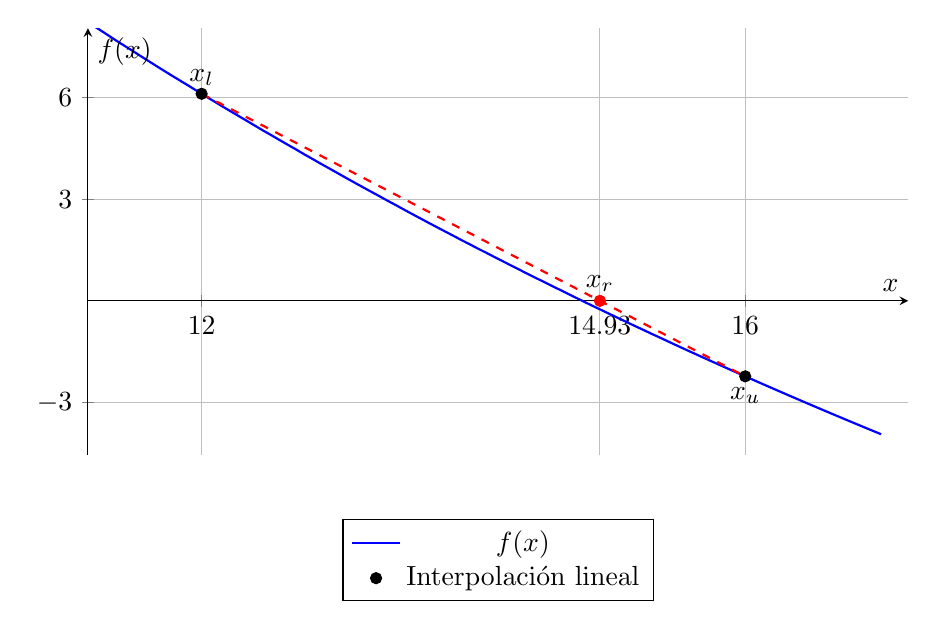
\begin{tikzpicture}
  \begin{axis}[
    width=12cm, height=7cm,
    domain=11:17,
    samples=100,
    axis lines=middle,
    xlabel={$x$}, ylabel={$f(x)$},
    grid=major,
    xtick={12,14.93,16},
    ytick={-3,0,3,6},
    ymin=-3.5, ymax=7,
    enlargelimits=true,
    legend style={at={(0.5,-0.15)}, anchor=north}
  ]
    % Función base (estilizada)
    \addplot[blue, thick] {668.06/x*(1 - exp(-0.146843*x)) - 40};
    \addlegendentry{$f(x)$}

    % Puntos xl y xu
    \addplot[only marks, mark=*] coordinates {(12, 6.1139)};
    \node at (axis cs:12,6.6) {$x_l$};

    \addplot[only marks, mark=*] coordinates {(16, -2.2303)};
    \node at (axis cs:16,-2.8) {$x_u$};

    % Línea de falsa posición
    \addplot[dashed, red, thick, domain=12:16] {((6.1139 - -2.2303)/(12 - 16))*(x - 16) + (-2.2303)};
    \addlegendentry{Interpolación lineal}

    % Punto xr
    \addplot[only marks, mark=*, red] coordinates {(14.9309, 0)};
    \node at (axis cs:14.9309,0.5) {$x_r$};

  \end{axis}
\end{tikzpicture}
\end{frame}



\begin{frame}{Ventajas de la Falsa Posición}
\begin{itemize}
  \item Más eficiente que la bisección en muchos casos.
  \item Aprovecha la magnitud de \( f(x_l) \) y \( f(x_u) \) para sesgar la estimación hacia la raíz.
  \item Convergencia más rápida si la función es aproximadamente lineal entre los extremos.
\end{itemize}
\end{frame}

\begin{frame}{Ejemplo 5: Primera Iteración}
\textbf{Problema:} Encontrar la raíz de
\[
  f(c) = \frac{668.06}{c}(1 - e^{-0.146843c}) - 40
\]
\begin{itemize}
  \item Intervalo inicial: \( x_l = 12 \), \( f(x_l) = 6.1139 \); \( x_u = 16 \), \( f(x_u) = -2.2303 \)
  \item Usando Falsa Posición:
  \[
    x_r = 16 - (-2.2303)(12 - 16)/\left(6.1139 + 2.2303\right) = 14.9309
  \]
  \item Error relativo verdadero: \( 0.88\% \)
\end{itemize}
\end{frame}

\begin{frame}{Segunda Iteración}
\begin{itemize}
  \item \( f(x_l) \cdot f(x_r) = 6.1139 \cdot (-0.2515) < 0 \)  $\Rightarrow$ \textbf{Raíz entre \( x_l = 12 \) y \( x_u = 14.9309 \)}
  \item Nueva estimación:
  \[
    x_r = 14.9309 - (-0.2515)(12 - 14.9309)/\left(6.1139 + 0.2515\right) = 14.8151
  \]
  \item \( \epsilon_t = 0.09\% \), \( \epsilon_a = 0.79\% \)
\end{itemize}
\end{frame}


\begin{frame}{Comparación: Falsa Posición vs Bisección}
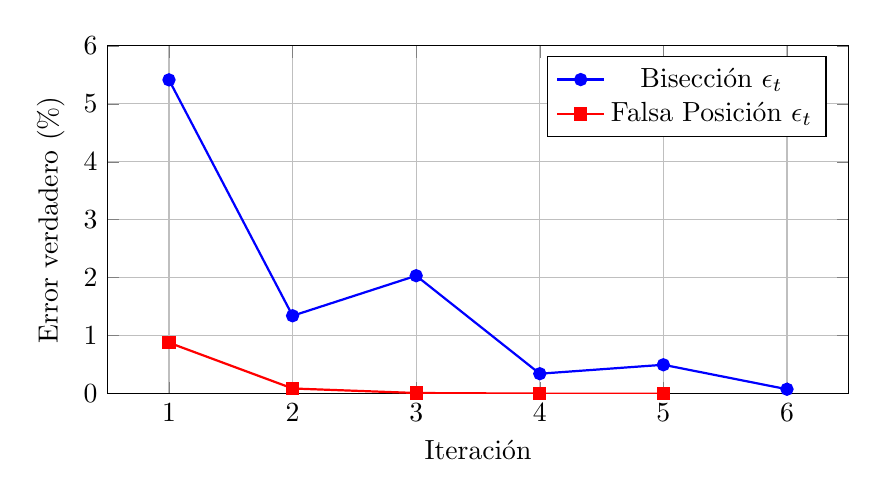
\begin{tikzpicture}
  \begin{axis}[
    width=11cm, height=6cm,
    xlabel={Iteración},
    ylabel={Error verdadero (\%)},
    xtick={1,2,3,4,5,6},
    ytick={0,1,...,6},
    legend pos=north east,
    grid=major,
    ymin=0, ymax=6
  ]
    \addplot[mark=*, blue, thick] coordinates {
      (1,5.413) (2,1.344) (3,2.035) (4,0.345) (5,0.499) (6,0.077)
    };
    \addlegendentry{Bisección $\epsilon_t$}

    \addplot[mark=square*, red, thick] coordinates {
      (1,0.88) (2,0.09) (3,0.012) (4,0.0015) (5,0.0002)
    };
    \addlegendentry{Falsa Posición $\epsilon_t$}
  \end{axis}
\end{tikzpicture}
\end{frame}

\begin{frame}{Tabla de Comparación de Errores}
\centering
%\small
\begin{tabular}{|c|c|c|}
\hline
\textbf{Iteración} & \textbf{Bisección $\epsilon_t$ (\%)} & \textbf{Falsa Posición $\epsilon_t$ (\%)} \\
\hline
1 & 5.413 & 0.88 \\
2 & 1.344 & 0.09 \\
3 & 2.035 & 0.012 \\
4 & 0.345 & 0.0015 \\
5 & 0.499 & 0.0002 \\
6 & 0.077 & -- \\
\hline
\end{tabular}
\end{frame}


\begin{frame}[fragile]{Pseudocódigo en Python: Falsa Posición}
\scriptsize
\begin{lstlisting}[style=mypython]
def falsa_posicion(f, xl, xu, es=0.001, max_iter=100):
    fl, fu = f(xl), f(xu)
    if fl * fu > 0:
        raise ValueError("No hay cambio de signo")
    xr_anterior = None
    for i in range(1, max_iter+1):
        xr = xu - fu * (xl - xu) / (fl - fu)
        fr = f(xr)

        if i == 1:
            ea = None
        elif xr != 0:
            ea = abs((xr - xr_anterior) / xr) * 100
        else:
            ea = float("inf")

        if fr == 0 or (ea is not None and ea < es):
            return xr, i, ea
        if fl * fr < 0:
            xu, fu = xr, fr
        else:
            xl, fl = xr, fr

        xr_anterior = xr
    return xr, max_iter, ea
\end{lstlisting}
\end{frame}



\begin{frame}{Ejemplo 6: Bisección vs Falsa Posición}
\small
\textbf{Función:} $f(x) = x^{10} - 1$ \\[0.5em]
\textbf{Intervalo:} $[0, 1.3]$

\begin{columns}
  \column{0.5\textwidth}
  \textbf{Bisección:}
  \begin{tabular}{|c|c|c|c|}
    \hline
    It & $x_r$ & $e_a$ (\%) & $e_t$ (\%) \\
    \hline
    1 & 0.65 & 100.0 & 35.0 \\
    2 & 0.975 & 33.3 & 2.5 \\
    3 & 1.1375 & 14.3 & 13.8 \\
    4 & 1.05625 & 7.7 & 5.6 \\
    5 & 1.015625 & 4.0 & 1.6 \\
    \hline
  \end{tabular}

  \column{0.5\textwidth}
  \textbf{Falsa Posición:}
  \begin{tabular}{|c|c|c|c|}
    \hline
    It & $x_r$ & $e_a$ (\%) & $e_t$ (\%) \\
    \hline
1 & 0.09430 & -- & 90.6 \\
    2 & 0.18176 & 48.1 & 81.8 \\
    3 & 0.26287 & 30.9 & 73.7 \\
    4 & 0.33811 & 22.3 & 66.2 \\
    5 & 0.40788 & 17.1 & 59.2 \\
    \hline
  \end{tabular}
\end{columns}
\end{frame}

\begin{frame}{Gráfica: Comparación de Convergencia}
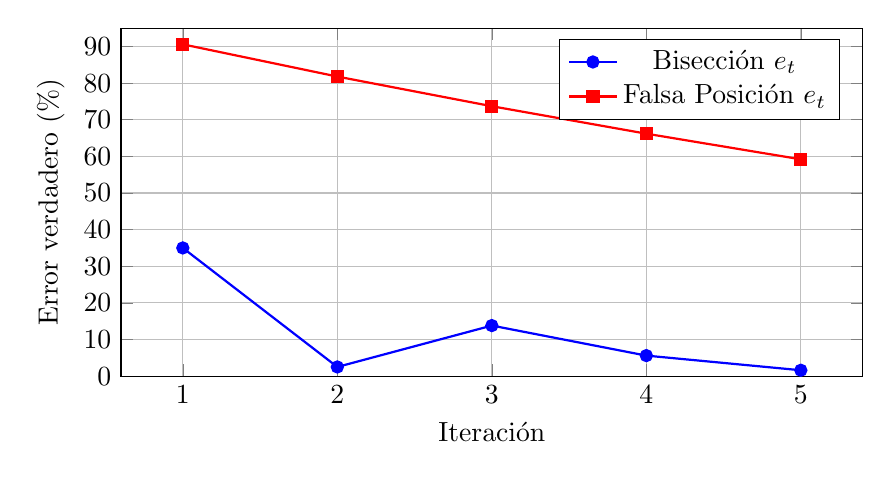
\begin{tikzpicture}
  \begin{axis}[
    width=11cm, height=6cm,
    xlabel={Iteración},
    ylabel={Error verdadero (\%)},
    xtick={1,2,3,4,5},
    ytick={0,10,20,30,40,50,60,70,80,90},
    legend pos=north east,
    grid=major,
    ymin=0, ymax=95
  ]
    \addplot[mark=*, blue, thick] coordinates {
      (1,35) (2,2.5) (3,13.8) (4,5.6) (5,1.6)
    };
    \addlegendentry{Bisección $e_t$}

    \addplot[mark=square*, red, thick] coordinates {
      (1,90.6) (2,81.8) (3,73.7) (4,66.2) (5,59.2)
    };
    \addlegendentry{Falsa Posición $e_t$}
  \end{axis}
\end{tikzpicture}
\end{frame}

\begin{frame}[fragile]{Pseudocódigo: Falsa Posición Modificada (1/2)}
\begin{lstlisting}[
  style=mypython,
  basicstyle=\scriptsize\ttfamily,
  frame=single
]
def falsa_pos_mod(f, xl, xu, es=0.01, imax=50):
    iter = 0
    fl, fu = f(xl), f(xu)
    if fl * fu > 0:
        raise ValueError("No hay cambio de signo")
    il, iu = 0, 0
    xr = xl
    ea = float("inf")
    while True:
        xrold = xr
        xr = xu - fu * (xl - xu) / (fl - fu)
        fr = f(xr)
        iter += 1
        if xr != 0:
            ea = abs((xr - xrold) / xr) * 100
        else:
            ea = float("inf")
\end{lstlisting}
\end{frame}

\begin{frame}[fragile]{Pseudocódigo: Falsa Posición Modificada (2/2)}
\begin{lstlisting}[
  style=mypython,
  basicstyle=\scriptsize\ttfamily,
  frame=single
]
        test = fl * fr
        if test < 0:
            xu, fu = xr, fr
            iu, il = 0, il + 1
            if il >= 2: fl /= 2
        elif test > 0:
            xl, fl = xr, fr
            il, iu = 0, iu + 1
            if iu >= 2: fu /= 2
        else:
            ea = 0
        if ea < es or iter >= imax:
            break
    return xr
\end{lstlisting}
\end{frame}


\begin{frame}{Conclusiones del Ejemplo 6}
\begin{itemize}
  \item La \textbf{falsa posición} puede ser ineficiente si uno de los extremos del intervalo permanece fijo.
  \item En funciones con curvatura pronunciada, la \textbf{bisección} puede superar a la falsa posición.
  \item La \textbf{falsa posición modificada} mejora la convergencia al evitar el estancamiento de extremos.
  \item Siempre se recomienda verificar la solución sustituyendo en la función original.
  \item Conocer el contexto del problema y graficar la función puede orientar sobre la mejor técnica.
\end{itemize}
\end{frame}

\subsection{Métodos Abiertos}
\begin{frame}{Métodos Abiertos: Introducción}
\begin{itemize}
  \item En los \textbf{métodos cerrados}, la raíz está contenida en un intervalo [\( x_l, x_u \)] conocido, y las aproximaciones siempre convergen hacia la raíz.
  \item En los \textbf{métodos abiertos}, se parte de uno o dos valores iniciales que no necesariamente encierran la raíz.
  \item Estos métodos pueden \textbf{divergir} (alejarse de la raíz) o \textbf{converger rápidamente}, dependiendo del valor inicial y la forma de la función.
  \item Cuando convergen, suelen hacerlo más rápido que los métodos cerrados.
\end{itemize}
\end{frame}

\subsubsection{Iteración de Punto Fijo}

\begin{frame}{Iteración Simple de Punto Fijo: Definición}
\begin{itemize}
  \item Los métodos abiertos emplean una fórmula para predecir la raíz.
  \item Se basa en reescribir la ecuación \( f(x) = 0 \) como:
  \[ x = g(x) \]
  \item Esta forma se logra con operaciones algebraicas simples.
  \item Permite calcular nuevas aproximaciones iterativas:
  \[ x_{i+1} = g(x_i) \]
\end{itemize}
\end{frame}

\begin{frame}{Iteración Simple de Punto Fijo: Ejemplos y Error}
\begin{itemize}
  \item Ejemplo algebraico con una raíz real positiva:
  \[ x^2 - x - 1 = 0 \Rightarrow x = \sqrt{x+1} \]
  \item Ejemplo trigonométrico:
  \[ \sin(x) = 0 \Rightarrow x = \sin(x) + x \]
  \item Error relativo aproximado:
  \[ \epsilon_a = \left| \frac{x_{i+1} - x_i}{x_{i+1}} \right| \times 100\% \]
\end{itemize}
\end{frame}


\begin{frame}{Métodos Abiertos vs Cerrados}
\begin{itemize}
  \item \textbf{Métodos cerrados:} requieren un intervalo [\( x_l, x_u \)] donde la raíz esté contenida.
  \item \textbf{Métodos abiertos:} usan uno o dos valores iniciales, no garantizan encerrar la raíz.
  \item Los métodos abiertos pueden \textbf{divergir} o \textbf{converger rápidamente}, dependiendo de los valores iniciales.
\end{itemize}
\end{frame}
\begin{frame}{Ejemplo 7: Iteración de Punto Fijo}
\textbf{Problema:} Usar iteración de punto fijo para encontrar la raíz de:
\[
  f(x) = e^{-x} - x, \quad \text{reorganizada como } x = g(x) = e^{-x}
\]
\textbf{Valor inicial:} \( x_0 = 0 \), \quad \textbf{Iteración:} \( x_{i+1} = e^{-x_i} \)

\vspace{0.5em}
\begin{columns}
\column{0.48\textwidth}
\begin{tabular}{|c|c|c|c|}
\hline
\textbf{i} & \( x_i \) & \( \epsilon_a \% \) & \( \epsilon_t \% \) \\
\hline
0 & 0.000000 & - & 100.0 \\
1 & 1.000000 & 100.0 & 76.3 \\
2 & 0.367879 & 171.8 & 35.1 \\
3 & 0.692201 & 46.9 & 22.1 \\
4 & 0.500473 & 38.3 & 11.8 \\
5 & 0.606244 & 17.4 & 6.89 \\
\hline
\end{tabular}

\column{0.48\textwidth}
\begin{tabular}{|c|c|c|c|}
\hline
\textbf{i} & \( x_i \) & \( \epsilon_a \% \) & \( \epsilon_t \% \) \\
\hline
6 & 0.545396 & 11.2 & 3.83 \\
7 & 0.579612 & 5.90 & 2.20 \\
8 & 0.560115 & 3.48 & 1.24 \\
9 & 0.571143 & 1.93 & 0.705 \\
10 & 0.564879 & 1.11 & 0.399 \\
\hline
\end{tabular}
\end{columns}

\vspace{0.5em}
\textbf{Conclusión:} La raíz se aproxima a \( x \approx 0.567143 \). El error disminuye progresivamente en cada iteración.
\end{frame}

\begin{frame}{Convergencia: Punto Fijo}
\begin{itemize}
  \item En el ejemplo anterior, el error relativo verdadero es aproximadamente proporcional al de la iteración anterior.
  \item Esta propiedad se conoce como \textbf{convergencia lineal}.
  \item Si \(0<|g'(x^*)|<1\), la convergencia local es lineal.
  \item Si \(g'(x^*)=0\), la convergencia puede ser superlineal.
  \item Los casos \(|g'(x^*)|=1\) requieren un análisis adicional.
  \item También se debe estudiar si el método \textbf{converge o diverge}.
\end{itemize}
\end{frame}

\begin{frame}{Método Gráfico de Dos Curvas}
\begin{itemize}
  \item Separar la ecuación \( f(x) = 0 \) como \( f_1(x) = f_2(x) \).
  \item Ejemplo: \( e^{-x} - x = 0 \) se convierte en:
  \begin{align*}
    y_1 &= x \\
    y_2 &= e^{-x}
  \end{align*}
  \item Las raíces son los puntos donde \( y_1 = y_2 \).
  \item Gráficamente: se intersectan las curvas \( y = x \) y \( y = e^{-x} \).
\end{itemize}
\end{frame}

\begin{frame}{Tabla del Método Gráfico}
\centering
\begin{tabular}{|c|c|c|}
\hline
\textbf{x} & \( y_1 = x \) & \( y_2 = e^{-x} \) \\
\hline
0.0 & 0.000 & 1.000 \\
0.2 & 0.200 & 0.819 \\
0.4 & 0.400 & 0.670 \\
0.6 & 0.600 & 0.549 \\
0.8 & 0.800 & 0.449 \\
1.0 & 1.000 & 0.368 \\
\hline
\end{tabular}

\vspace{1em}
\begin{center}
\textbf{Intersección:} Aproximadamente en \( x = 0.57 \)
\end{center}
\end{frame}

\begin{frame}{Gráfico: Método de Dos Curvas}
\centering
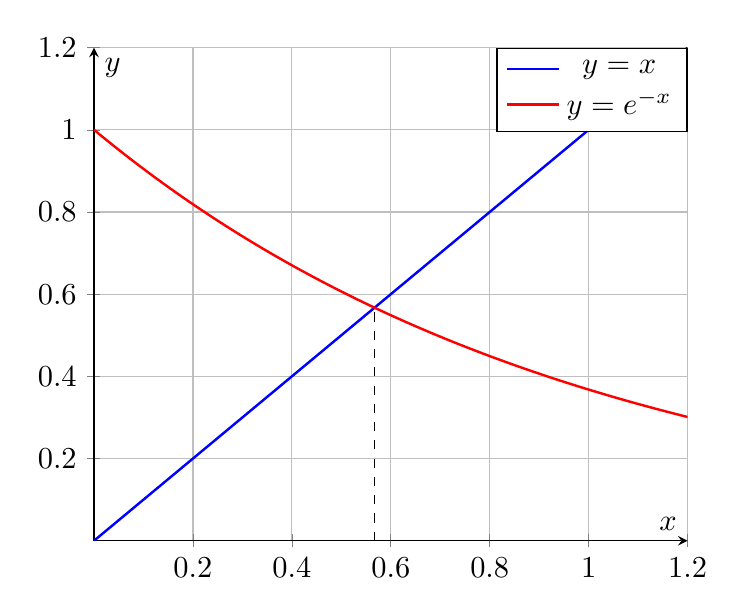
\begin{tikzpicture}[scale=1.1]
  \begin{axis}[
    axis lines=middle,
    xmin=0, xmax=1.2,
    ymin=0, ymax=1.2,
    xlabel={$x$}, ylabel={$y$},
    legend style={at={(1,1)}, anchor=north east},
    grid=major
  ]
  \addplot[domain=0:1.2, samples=100, thick, blue] {x};
  \addplot[domain=0:1.2, samples=100, thick, red] {exp(-x)};
  \addlegendentry{$y = x$}
  \addlegendentry{$y = e^{-x}$}
  \draw[dashed] (axis cs:0.567,0) -- (axis cs:0.567,0.567);
  \node[below] at (axis cs:0.567,0) {$\approx 0.57$};
  \end{axis}
\end{tikzpicture}
\end{frame}

\begin{frame}{Convergencia y Divergencia Gráfica}
\begin{itemize}
  \item Se grafica \( y_1 = x \) y \( y_2 = g(x) \).
  \item El proceso iterativo: de \( x_i \) a \( g(x_i) \), luego a \( x_{i+1} \).
  \item \textbf{Convergente:} se acerca a la raíz en cada iteración.
  \item \textbf{Divergente:} se aleja de la raíz.
  \item La convergencia ocurre si: \( |g'(x)| < 1 \)
\end{itemize}
\end{frame}


%========================================================
% DEMOSTRACIÓN DE LA CONVERGENCIA
%========================================================

\begin{frame}{Convergencia de la Iteración de Punto Fijo}

\begin{itemize}
  \item La iteración de punto fijo está definida por: \(x_{i+1}=g(x_i)\)
  \item Supongamos que \(x^*\) es un punto fijo: \(x^*=g(x^*)\)
  \item Restando ambas expresiones: \(x^*-x_{i+1}=g(x^*)-g(x_i) \)
  \item Por el teorema del valor medio, existe un punto
  \(\xi_i\) entre \(x_i\) y \(x^*\) tal que:
  \[
    g(x^*)-g(x_i)=g'(\xi_i)(x^*-x_i).
  \]

  \item Si \(E_{t,i}=x^*-x_i\), entonces:
  \[
    E_{t,i+1}=g'(\xi_i)E_{t,i}.
  \]

  \item Por tanto:
  \[
    |E_{t,i+1}|=|g'(\xi_i)|\,|E_{t,i}|.
  \]

  \item Si \(|g'(x)|\leq k<1\) en un entorno de \(x^*\),
  los errores disminuyen y el método converge localmente.
\end{itemize}

\end{frame}


%========================================================
% CLASIFICACIÓN Y ALGORITMO
%========================================================

\begin{frame}[fragile]{Análisis de Error y Algoritmo de Punto Fijo}

\begin{itemize}
  \item Si \(0<g'(x^*)<1\): convergencia monótona.
  \item Si \(-1<g'(x^*)<0\): convergencia oscilatoria.
  \item Si \(g'(x^*)>1\): divergencia monótona.
  \item Si \(g'(x^*)<-1\): divergencia oscilatoria.
  \item Cerca del punto fijo: \(E_{t,i+1}\approx g'(x^*)E_{t,i}.\)
\end{itemize}

\begin{lstlisting}[
  style=mypython,
  basicstyle=\scriptsize\ttfamily,
  frame=single
]
def punto_fijo(g, x0, es=0.001, imax=50):
    for i in range(imax):
        x1 = g(x0)
        denominador = max(abs(x1), 1e-12)
        ea = abs((x1 - x0) / denominador) * 100
        if ea < es:
            return x1, i + 1, ea
        x0 = x1
    return x1, imax, ea
\end{lstlisting}

\end{frame}


%========================================================
% CASO 1: CONVERGENCIA MONÓTONA
%========================================================

\begin{frame}{Convergencia de Punto Fijo: Caso Monótono Convergente}

\centering
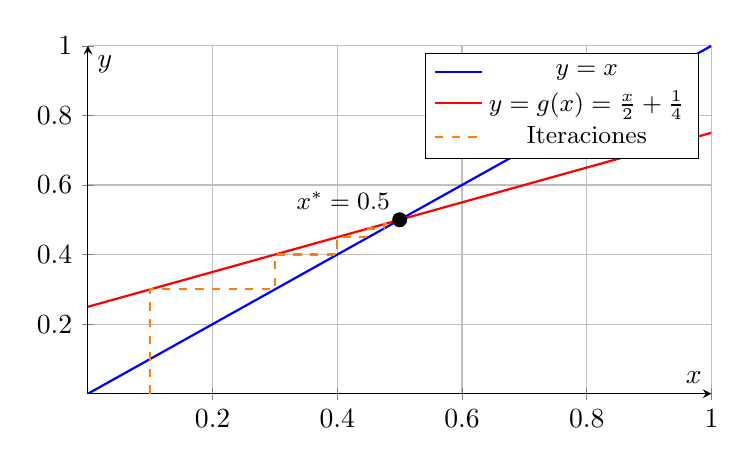
\begin{tikzpicture}
  \begin{axis}[
    width=9.5cm,
    height=6cm,
    axis lines=middle,
    xmin=0, xmax=1,
    ymin=0, ymax=1,
    xlabel={$x$},
    ylabel={$y$},
    grid=major,
    legend style={
      at={(0.98,0.98)},
      anchor=north east,
      font=\small
    }
  ]

  % Recta y=x
  \addplot[
    domain=0:1,
    samples=100,
    thick,
    blue
  ] {x};
  \addlegendentry{$y=x$}

  % Función de iteración
  \addplot[
    domain=0:1,
    samples=100,
    thick,
    red
  ] {0.5*x + 0.25};
  \addlegendentry{$y=g(x)=\frac{x}{2}+\frac14$}

  % Diagrama de telaraña desde x_0=0.1
  \addplot[
    thick,
    dashed,
    orange
  ] coordinates {
    (0.1,0)
    (0.1,0.3)
    (0.3,0.3)
    (0.3,0.4)
    (0.4,0.4)
    (0.4,0.45)
    (0.45,0.45)
    (0.45,0.475)
    (0.475,0.475)
    (0.475,0.4875)
    (0.4875,0.4875)
    (0.4875,0.49375)
    (0.49375,0.49375)
  };
  \addlegendentry{Iteraciones}

  % Punto fijo
  \addplot[
    only marks,
    mark=*,
    mark size=2.5pt,
    black
  ] coordinates {
    (0.5,0.5)
  };

  \node[
    above left,
    font=\small
  ] at (axis cs:0.5,0.5)
    {$x^*=0.5$};

  \node[
    below,
    font=\small
  ] at (axis cs:0.1,0)
    {$x_0=0.1$};

  \end{axis}
\end{tikzpicture}

\textbf{Comentario:}
La convergencia es monótona cuando \(0<g'(x^*)<1\).

\textbf{Ejemplo:}
Para \(g(x)=\frac{x}{2}+\frac14\),
\(
g'(x)=\frac12,
\quad
|g'(x)|=\frac12<1.
\)
Por tanto, el método converge monótonamente hacia \(x^*=0.5\).

\end{frame}


%========================================================
% CASO 2: CONVERGENCIA OSCILATORIA
%========================================================

\begin{frame}{Convergencia de Punto Fijo: Caso Oscilatorio Convergente}

\centering
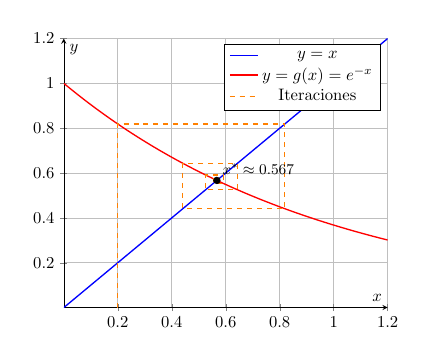
\begin{tikzpicture}[scale=.6]
  \begin{axis}[
    axis lines=middle,
    xmin=0, xmax=1.2,
    ymin=0, ymax=1.2,
    xlabel={$x$},
    ylabel={$y$},
    legend style={
      at={(0.98,0.98)},
      anchor=north east
    },
    grid=major
  ]

  % Recta y=x
  \addplot[
    domain=0:1.2,
    samples=100,
    thick,
    blue
  ] {x};
  \addlegendentry{$y=x$}

  % Función de iteración
  \addplot[
    domain=0:1.2,
    samples=100,
    thick,
    red
  ] {exp(-x)};
  \addlegendentry{$y=g(x)=e^{-x}$}

  % Diagrama de telaraña desde x_0=0.2
  \addplot[
    thick,
    dashed,
    orange
  ] coordinates {
    (0.2,0)
    (0.2,0.8187)
    (0.8187,0.8187)
    (0.8187,0.4410)
    (0.4410,0.4410)
    (0.4410,0.6434)
    (0.6434,0.6434)
    (0.6434,0.5255)
    (0.5255,0.5255)
    (0.5255,0.5912)
    (0.5912,0.5912)
    (0.5912,0.5538)
    (0.5538,0.5538)
    (0.5538,0.5747)
    (0.5747,0.5747)
  };
  \addlegendentry{Iteraciones}

  % Punto fijo
  \addplot[
    only marks,
    mark=*,
    mark size=2pt,
    black
  ] coordinates {
    (0.567143,0.567143)
  };

  \node[
    below,
    font=\small
  ] at (axis cs:0.2,0)
    {$x_0=0.2$};

  \node[
    above right,
    font=\small
  ] at (axis cs:0.567143,0.567143)
    {$x^*\approx0.567$};

  \end{axis}
\end{tikzpicture}

La convergencia es oscilatoria cuando
\(-1<g'(x^*)<0\). Las aproximaciones alternan alrededor del
punto fijo y se acercan progresivamente a él.

\textbf{Ejemplo:}
Para \(g(x)=e^{-x}\), \(g'(x)=-e^{-x}\). En \(x^*\approx0.567\),
\[
g'(x^*)\approx-0.567,
\qquad
|g'(x^*)|\approx0.567<1.
\]
Por tanto, el método converge de manera oscilatoria.

\end{frame}


%========================================================
% CASO 3: DIVERGENCIA MONÓTONA
%========================================================

\begin{frame}{Convergencia de Punto Fijo: Caso Monótono Divergente}

\centering
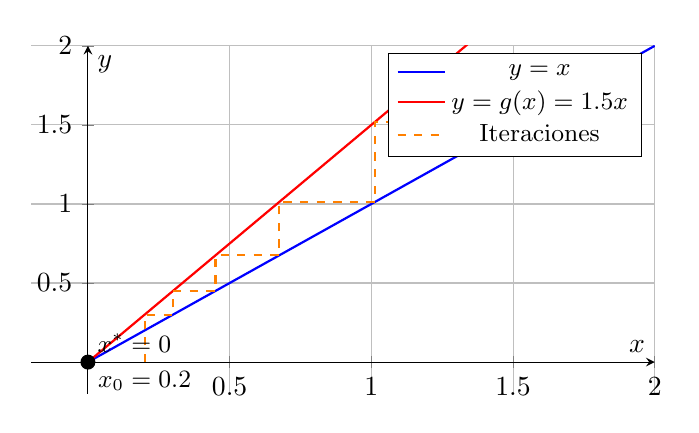
\begin{tikzpicture}
  \begin{axis}[
    width=9.5cm,
    height=6cm,
    axis lines=middle,
    xmin=-0.2, xmax=2,
    ymin=-0.2, ymax=2,
    xlabel={$x$},
    ylabel={$y$},
    grid=major,
    legend style={
      at={(0.98,0.98)},
      anchor=north east,
      font=\small
    }
  ]

  % Recta y=x
  \addplot[
    domain=0:2,
    samples=100,
    thick,
    blue
  ] {x};
  \addlegendentry{$y=x$}

  % Función de iteración
  \addplot[
    domain=0:1.34,
    samples=100,
    thick,
    red
  ] {1.5*x};
  \addlegendentry{$y=g(x)=1.5x$}

  % Diagrama de telaraña desde x_0=0.2
  \addplot[
    thick,
    dashed,
    orange
  ] coordinates {
    (0.2,0)
    (0.2,0.3)
    (0.3,0.3)
    (0.3,0.45)
    (0.45,0.45)
    (0.45,0.675)
    (0.675,0.675)
    (0.675,1.0125)
    (1.0125,1.0125)
    (1.0125,1.51875)
    (1.51875,1.51875)
  };
  \addlegendentry{Iteraciones}

  % Punto fijo
  \addplot[
    only marks,
    mark=*,
    mark size=2.5pt,
    black
  ] coordinates {
    (0,0)
  };

  \node[
    above right,
    font=\small
  ] at (axis cs:0,0)
    {$x^*=0$};

  \node[
    below,
    font=\small
  ] at (axis cs:0.2,0)
    {$x_0=0.2$};

  \end{axis}
\end{tikzpicture}

\textbf{Comentario:}
Cuando \(g'(x^*)>1\), las aproximaciones permanecen del mismo
lado del punto fijo, pero se alejan progresivamente de él.

\textbf{Ejemplo:}
Para \(g(x)=1.5x\),
\(
g'(x)=1.5,
\quad
|g'(x)|=1.5>1.
\)
Por tanto, el método diverge monótonamente desde \(x_0=0.2\).

\end{frame}


%========================================================
% CASO 4: DIVERGENCIA OSCILATORIA
%========================================================

\begin{frame}{Convergencia de Punto Fijo: Caso Oscilatorio Divergente}

\centering
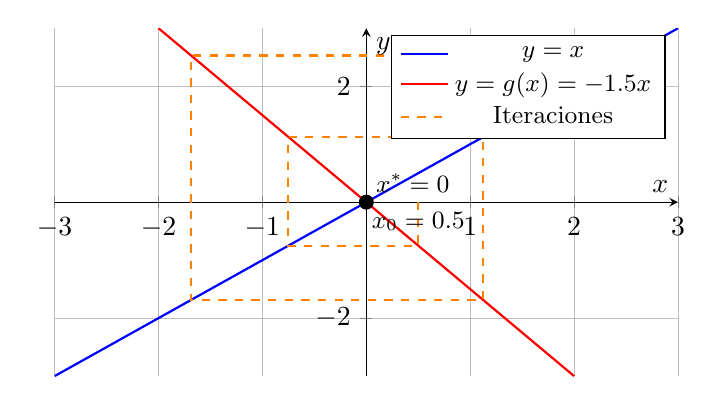
\begin{tikzpicture}
  \begin{axis}[
    width=9.5cm,
    height=6cm,
    axis lines=middle,
    xmin=-3, xmax=3,
    ymin=-3, ymax=3,
    xlabel={$x$},
    ylabel={$y$},
    grid=major,
    legend style={
      at={(0.98,0.98)},
      anchor=north east,
      font=\small
    }
  ]

  % Recta y=x
  \addplot[
    domain=-3:3,
    samples=100,
    thick,
    blue
  ] {x};
  \addlegendentry{$y=x$}

  % Función de iteración
  \addplot[
    domain=-2:2,
    samples=100,
    thick,
    red
  ] {-1.5*x};
  \addlegendentry{$y=g(x)=-1.5x$}

  % Diagrama de telaraña desde x_0=0.5
  \addplot[
    thick,
    dashed,
    orange
  ] coordinates {
    (0.5,0)
    (0.5,-0.75)
    (-0.75,-0.75)
    (-0.75,1.125)
    (1.125,1.125)
    (1.125,-1.6875)
    (-1.6875,-1.6875)
    (-1.6875,2.53125)
    (2.53125,2.53125)
  };
  \addlegendentry{Iteraciones}

  % Punto fijo
  \addplot[
    only marks,
    mark=*,
    mark size=2.5pt,
    black
  ] coordinates {
    (0,0)
  };

  \node[
    above right,
    font=\small
  ] at (axis cs:0,0)
    {$x^*=0$};

  \node[
    below,
    font=\small
  ] at (axis cs:0.5,0)
    {$x_0=0.5$};

  \end{axis}
\end{tikzpicture}

\textbf{Comentario:}
Cuando \(g'(x^*)<-1\), el método diverge de forma oscilatoria.
Las aproximaciones alternan a ambos lados del punto fijo y se
alejan progresivamente de él.

\textbf{Ejemplo:}
Para \(g(x)=-1.5x\),
\(
g'(x)=-1.5,
\quad
|g'(x)|=1.5>1.
\)
Por tanto, las iteraciones divergen de manera oscilatoria.

\end{frame}


%========================================================
% MÉTODO DE NEWTON-RAPHSON: CONCEPTO
%========================================================

\subsubsection{Método de Newton-Raphson}

\begin{frame}{Método de Newton-Raphson}

\textbf{Concepto:}
Parte de una estimación inicial \(x_i\) y utiliza la recta tangente
en el punto \(\bigl(x_i,f(x_i)\bigr)\) para obtener una mejor
aproximación de la raíz.

\vspace{0.8em}

\textbf{Fórmula:}
\[
x_{i+1}
=
x_i-\frac{f(x_i)}{f'(x_i)},
\qquad f'(x_i)\neq 0.
\]

\vspace{0.8em}

\textbf{Interpretación geométrica:}
La nueva aproximación \(x_{i+1}\) es el punto donde la recta
tangente a \(f(x)\) en \(x_i\) cruza el eje \(x\).

\vspace{0.5em}

\textbf{Ventaja:}
Presenta convergencia rápida cuando la estimación inicial está
suficientemente cerca de una raíz simple y \(f'(x^*)\neq0\).

\end{frame}


%========================================================
% EJEMPLO NUMÉRICO
%========================================================

\begin{frame}{Ejemplo: Método de Newton-Raphson}

\textbf{Función:}
\[
f(x)=e^{-x}-x,
\qquad
f'(x)=-e^{-x}-1.
\]

\textbf{Fórmula de iteración:}
\[
x_{i+1}
=
x_i-\frac{e^{-x_i}-x_i}{-e^{-x_i}-1}.
\]

\centering
\small

\begin{tabular}{|c|c|c|}
\hline
\textbf{\(i\)} & \(\boldsymbol{x_i}\) &
\(\boldsymbol{\varepsilon_{t,i}(\%)}\) \\ \hline
0 & 0.000000000 & 100.000000 \\ 
1 & 0.500000000 & 11.838000 \\ 
2 & 0.566311003 & 0.146750 \\ 
3 & 0.567143165 & \(2.21\times10^{-5}\) \\ 
4 & 0.567143290 & \(<10^{-8}\) \\ \hline
\end{tabular}

\vspace{0.4em}

\raggedright
Para calcular el error verdadero se utilizó \( x^*\approx0.567143290.\)

\end{frame}


%========================================================
% CONVERGENCIA
%========================================================

\begin{frame}{Convergencia del Método de Newton-Raphson}
\textbf{Criterio de terminación:}
\[
\varepsilon_a
=
\left|
\frac{x_{i+1}-x_i}{x_{i+1}}
\right|100\%
<
\varepsilon_s.
\]
\textbf{Convergencia cuadrática:}
\(
|E_{t,i+1}|
=
\mathcal{O}\left(|E_{t,i}|^2\right).
\)
\begin{itemize}
  \item El número de cifras correctas aumenta rápidamente.
  \item Aproximadamente se duplica el número de cifras correctas
        en cada iteración, una vez alcanzada la región de convergencia.
  \item La raíz debe ser simple y debe cumplirse \(f'(x^*)\neq0\).
  \item La aproximación inicial debe estar suficientemente cerca
        de la raíz.
\end{itemize}
\textbf{Comparación:}
Newton-Raphson suele presentar convergencia cuadrática, mientras
que la iteración de punto fijo estándar generalmente presenta
convergencia lineal.

\end{frame}


%========================================================
% ANÁLISIS DEL ERROR
%========================================================

\begin{frame}{Análisis del Error en Newton-Raphson}

\textbf{Problema:}
Verificar la convergencia cuadrática del método de Newton-Raphson.

\vspace{0.5em}

Si se define
\[
E_{t,i}=x^*-x_i,
\]
entonces, cerca de una raíz simple,
\[
E_{t,i+1}
\approx
-\frac{f''(x^*)}{2f'(x^*)}E_{t,i}^2.
\]

Para analizar solamente la magnitud del error:
\[
|E_{t,i+1}|
\approx
\left|
\frac{f''(x^*)}{2f'(x^*)}
\right|
|E_{t,i}|^2.
\]

\textbf{Función analizada:}
\[
f(x)=e^{-x}-x,
\qquad
x^*\approx0.56714329.
\]

\end{frame}


%========================================================
% CONSTANTE ASINTÓTICA DEL ERROR
%========================================================

\begin{frame}{Análisis del Error: Constante Asintótica}
\textbf{Derivadas:}
\[
f'(x)=-e^{-x}-1,
\qquad
f''(x)=e^{-x}.
\]
Evaluando en \(x^*=0.56714329\):
\[
f'(x^*)=-1.56714329,
\qquad
f''(x^*)=0.56714329.
\]
\textbf{Coeficiente con signo:}
\[
-\frac{f''(x^*)}{2f'(x^*)}
=
-\frac{0.56714329}{2(-1.56714329)}
\approx0.18095.
\]
\textbf{Constante para la magnitud del error:}
\[
C=
\left|
\frac{f''(x^*)}{2f'(x^*)}
\right|
\approx0.18095.
\]
Por tanto:
\[
|E_{t,i+1}|
\approx
0.18095\,|E_{t,i}|^2.
\]

\end{frame}


%========================================================
% COMPARACIÓN DE ERRORES
%========================================================

\begin{frame}{Análisis del Error: Verificación Numérica}

\small

Los errores verdaderos absolutos son:
\[
|E_{t,i}|=|x^*-x_i|.
\]

\centering

\begin{tabular}{|c|c|c|c|}
\hline
\(\boldsymbol{i}\) &
\(\boldsymbol{|E_{t,i}|}\) &
\(\boldsymbol{0.18095|E_{t,i}|^2}\) &
\(\boldsymbol{|E_{t,i+1}|}\) \\ \hline
0 &
\(5.6714\times10^{-1}\) &
\(5.82\times10^{-2}\) &
\(6.7143\times10^{-2}\) \\

1 &
\(6.7143\times10^{-2}\) &
\(8.16\times10^{-4}\) &
\(8.3229\times10^{-4}\) \\

2 &
\(8.3229\times10^{-4}\) &
\(1.253\times10^{-7}\) &
\(1.254\times10^{-7}\) \\ \hline
\end{tabular}

\vspace{0.7em}

\raggedright
\textbf{Interpretación:}
La estimación del error mejora a medida que \(x_i\) se aproxima
a la raíz. Esto ocurre porque la expresión del error es asintótica.

\vspace{0.5em}

\textbf{Conclusión:}
El error de la siguiente iteración es aproximadamente proporcional
al cuadrado del error actual, lo que confirma la convergencia
cuadrática del método.

\end{frame}


%========================================================
% DEDUCCIÓN DE LA FÓRMULA
%========================================================

\begin{frame}{Deducción mediante la Serie de Taylor}

\textbf{Objetivo:}
Deducir la fórmula de Newton-Raphson utilizando una aproximación
lineal de \(f(x)\) alrededor de \(x_i\).
La serie de Taylor es:
\(
f(x)
=
f(x_i)+f'(x_i)(x-x_i)
+\frac{f''(\xi_i)}{2}(x-x_i)^2,
\)
donde \(\xi_i\) se encuentra entre \(x_i\) y \(x\).

Al despreciar los términos de segundo orden y superiores:
\[
f(x)\approx f(x_i)+f'(x_i)(x-x_i).
\]

Se busca el punto \(x_{i+1}\) donde esta aproximación lineal
es igual a cero:
\[
0=f(x_i)+f'(x_i)(x_{i+1}-x_i).
\]

Despejando:
\[
\boxed{
x_{i+1}
=
x_i-\frac{f(x_i)}{f'(x_i)}
}
\]

\end{frame}


%========================================================
% DEDUCCIÓN DEL ERROR
%========================================================

\begin{frame}{Deducción de la Ecuación del Error}

Aplicando Taylor en \(x_i\) y evaluando en la raíz \(x^*\):
\[
0
=
f(x_i)+f'(x_i)(x^*-x_i)
+\frac{f''(\xi_i)}{2}(x^*-x_i)^2.
\]

La ecuación de Newton-Raphson es:
\(
0
=
f(x_i)+f'(x_i)(x_{i+1}-x_i).
\)

Restando ambas expresiones:
\[
0
=
f'(x_i)(x^*-x_{i+1})
+\frac{f''(\xi_i)}{2}(x^*-x_i)^2.
\]

Definiendo
\[
E_{t,i}=x^*-x_i,
\qquad
E_{t,i+1}=x^*-x_{i+1},
\]
se obtiene:
\[
E_{t,i+1}
=
-\frac{f''(\xi_i)}{2f'(x_i)}E_{t,i}^2.
\]

\end{frame}


%========================================================
% CONCLUSIÓN DE LA DEDUCCIÓN
%========================================================

\begin{frame}{Condiciones de Convergencia Cuadrática}

Cuando \(x_i\to x^*\), también se cumple que
\[
\xi_i\to x^*.
\]

Por tanto:
\[
E_{t,i+1}
\approx
-\frac{f''(x^*)}{2f'(x^*)}E_{t,i}^2.
\]

El método presenta convergencia cuadrática si:

\begin{itemize}
  \item \(x^*\) es una raíz simple.
  \item \(f'(x^*)\neq0\).
  \item \(f\) posee primera y segunda derivada continuas
        cerca de \(x^*\).
  \item La aproximación inicial \(x_0\) está suficientemente
        cerca de la raíz.
\end{itemize}

\textbf{Conclusión:}
Bajo estas condiciones, el error disminuye aproximadamente como
el cuadrado del error anterior.

\end{frame}


%========================================================
% GRÁFICO DEL MÉTODO
%========================================================

\begin{frame}{Interpretación Geométrica del Método}

\centering

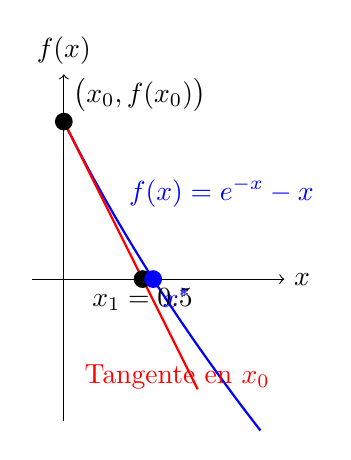
\begin{tikzpicture}[scale=2]

  % Ejes
  \draw[->] (-0.2,0) -- (1.4,0)
    node[right] {$x$};

  \draw[->] (0,-0.9) -- (0,1.3)
    node[above] {$f(x)$};

  % Función
  \draw[
    domain=0:1.25,
    samples=150,
    smooth,
    variable=\x,
    blue,
    thick
  ]
  plot ({\x},{exp(-\x)-\x});

  % Tangente en x0=0
  % f(0)=1 y f'(0)=-2
  \draw[
    domain=0:0.85,
    samples=2,
    variable=\x,
    red,
    thick
  ]
  plot ({\x},{1-2*\x});

  % Línea vertical desde x0
  \draw[dashed]
    (0,0) -- (0,1);

  % Punto inicial sobre la curva
  \filldraw[black]
    (0,1) circle (1.5pt)
    node[above right] {\(\bigl(x_0,f(x_0)\bigr)\)};

  % Primera aproximación
  \filldraw[black]
    (0.5,0) circle (1.5pt)
    node[below] {\(x_1=0.5\)};

  % Raíz verdadera
  \filldraw[blue]
    (0.567143,0) circle (1.5pt)
    node[below right] {\(x^*\)};

  % Etiquetas
  \node[blue] at (1.0,0.55)
    {\(f(x)=e^{-x}-x\)};

  \node[red] at (0.72,-0.62)
    {Tangente en \(x_0\)};

\end{tikzpicture}

\vspace{0.4em}

La tangente en \(x_0=0\) cruza el eje \(x\) en
\[
x_1
=
x_0-\frac{f(x_0)}{f'(x_0)}
=
0-\frac{1}{-2}
=
0.5.
\]

\end{frame}


%========================================================
% CÓDIGO EN PYTHON
%========================================================

\begin{frame}[fragile]{Algoritmo de Newton-Raphson en Python}

\begin{lstlisting}[
  style=mypython,
  basicstyle=\scriptsize\ttfamily,
  frame=single
]
def newton_raphson(f, df, x0, tol_x=1e-8,tol_f=1e-8,imax=50):
    x = x0
    for i in range(imax):
        derivada = df(x)
        if abs(derivada) < 1e-12:
            raise ValueError(
                "Derivada nula o muy pequena"
            )
        x_new = x - f(x) / derivada
        ea = abs(x_new - x) / max(
            abs(x_new), 1e-12
        ) * 100
        if ea < tol_x and abs(f(x_new)) < tol_f:
            return x_new, i + 1, ea
        x = x_new
    return x, imax, ea
\end{lstlisting}

\end{frame}


%========================================================
% DESVENTAJAS
%========================================================

\begin{frame}{Desventajas del Método de Newton-Raphson}

\textbf{Puntos clave:}

\begin{itemize}
  \item Depende de la selección de la aproximación inicial.
  \item Puede converger hacia una raíz diferente de la esperada.
  \item Puede divergir o entrar en ciclos para ciertos valores iniciales.
  \item Si \(f'(x_i)\approx0\), puede producir saltos muy grandes.
  \item Si \(f'(x_i)=0\), la fórmula no está definida.
  \item En raíces múltiples, la convergencia generalmente se reduce
        de cuadrática a lineal.
  \item Requiere calcular y evaluar la derivada de la función.
\end{itemize}

\end{frame}


%========================================================
% EJEMPLO DE MALA APROXIMACIÓN INICIAL
%========================================================

\begin{frame}{Ejemplo: Derivada Pequeña y Salto Inicial}

\textbf{Función:}
\[
f(x)=x^{10}-1,
\qquad
f'(x)=10x^9.
\]

\textbf{Fórmula de Newton-Raphson:}
\[
x_{i+1}
=
x_i-\frac{x_i^{10}-1}{10x_i^9}.
\]

Para \(x_0=0.5\):
\[
f'(0.5)=10(0.5)^9\approx0.01953.
\]

Como la derivada es pequeña, la primera iteración produce
un salto muy grande:
\[
x_1
=
0.5-\frac{0.5^{10}-1}{10(0.5)^9}
=
51.65.
\]

\end{frame}


%========================================================
% ITERACIONES DEL EJEMPLO
%========================================================

\begin{frame}{Ejemplo: Comportamiento de las Iteraciones}

\centering

\begin{tabular}{|c|c|}
\hline
\textbf{Iteración} & \(\boldsymbol{x_i}\) \\ \hline
0 & 0.500000 \\ 
1 & 51.650000 \\ 
2 & 46.485000 \\ 
3 & 41.836500 \\ 
4 & 37.652850 \\ 
5 & 33.887565 \\ 
\(\vdots\) & \(\vdots\) \\ 
 & \(x_i\longrightarrow1\) \\ \hline
\end{tabular}

\raggedright
\textbf{Interpretación:}
La derivada pequeña en \(x_0=0.5\) provoca que el método se aleje
inicialmente de la raíz. Después del salto, las aproximaciones
descienden lentamente durante varias iteraciones. Cuando las aproximaciones se acercan a la raíz simple \(x^*=1\), el método recupera su comportamiento cuadrático.

\end{frame}


%========================================================
% DIFICULTADES ADICIONALES
%========================================================

\begin{frame}{Dificultades Adicionales}

\textbf{Problemas comunes:}

\begin{itemize}
  \item \textbf{Derivada cercana a cero:}
        puede generar pasos excesivamente grandes.

  \item \textbf{División por cero:}
        ocurre si \(f'(x_i)=0\).

  \item \textbf{Oscilaciones o ciclos:}
        las aproximaciones pueden repetirse sin acercarse a una raíz.

  \item \textbf{Divergencia:}
        las aproximaciones pueden alejarse progresivamente.

  \item \textbf{Varias raíces:}
        diferentes valores iniciales pueden conducir a raíces distintas.

  \item \textbf{Raíces múltiples:}
        el método estándar generalmente presenta convergencia lineal.
\end{itemize}

\end{frame}


%========================================================
% RECOMENDACIONES
%========================================================

\begin{frame}{Recomendaciones y Mejoras}

\textbf{Buenas prácticas para mejorar el método:}

\begin{enumerate}
  \item Graficar la función para seleccionar una aproximación inicial.
  \item Establecer un número máximo de iteraciones.
  \item Verificar si \(|f'(x_i)|\) es demasiado pequeño.
  \item Controlar el cambio entre aproximaciones:
  \[
    |x_{i+1}-x_i|<\varepsilon_x.
  \]
  \item Verificar también el residuo:
  \[
    |f(x_{i+1})|<\varepsilon_f.
  \]
  \item Informar si el método termina sin alcanzar las tolerancias.
\end{enumerate}

\textbf{Conclusión:}
Newton-Raphson es un método potente y rápido, pero requiere
validaciones numéricas y una adecuada selección de \(x_0\).

\end{frame}



%========================================================
% MÉTODO DE LA SECANTE: CONCEPTO
%========================================================

\subsubsection{Métodos de la Secante}

\begin{frame}{Método de la Secante}

\textbf{Motivación:}
Cuando la derivada es difícil de obtener, puede aproximarse mediante
la pendiente de una recta secante:
\[
f'(x_i)
\approx
\frac{f(x_i)-f(x_{i-1})}{x_i-x_{i-1}}.
\]
\textbf{Fórmula iterativa:}
\[
\boxed{
x_{i+1}
=
x_i
-
f(x_i)
\frac{x_i-x_{i-1}}
{f(x_i)-f(x_{i-1})}
}
\]

\begin{itemize}
  \item Requiere dos valores iniciales diferentes:
        \(x_{-1}\) y \(x_0\).
  \item No requiere calcular explícitamente \(f'(x)\).
  \item No exige que \(f(x)\) cambie de signo entre los valores iniciales.
  \item Es un \textbf{método abierto}; por tanto, puede divergir.
  \item Requiere que\(
  f(x_i)-f(x_{i-1})\neq0.
  \)
\end{itemize}

\end{frame}


%========================================================
% EJEMPLO DEL MÉTODO DE LA SECANTE: PARTE 1
%========================================================

\begin{frame}{Ejemplo: Método de la Secante}

\textbf{Función:}
\(
f(x)=e^{-x}-x.
\)

\textbf{Raíz de referencia:}
\(
x^*\approx0.56714329.
\)

\textbf{Valores iniciales:}
\(
x_{-1}=0,
\qquad
x_0=1.
\)

Evaluaciones iniciales:
\(
f(x_{-1})=f(0)=1,
\)

\[
f(x_0)=f(1)=e^{-1}-1\approx-0.63212056.
\]
Primera aproximación:
\[
x_1
=
1
-
(-0.63212056)
\frac{1-0}
{-0.63212056-1}
\approx0.61269984.
\]

\[
\varepsilon_{t,1}
=
\left|
\frac{x^*-x_1}{x^*}
\right|100\%
\approx8.0326\%.
\]

\end{frame}


%========================================================
% EJEMPLO DEL MÉTODO DE LA SECANTE: PARTE 2
%========================================================

\begin{frame}{Ejemplo: Método de la Secante}

Para la segunda iteración:

\(
f(x_1)
=
f(0.61269984)
\approx-0.07081395.
\)
\[
x_2
=
x_1
-
f(x_1)
\frac{x_1-x_0}
{f(x_1)-f(x_0)}.
\]
\[
x_2
=
0.61269984
-
(-0.07081395)
\frac{0.61269984-1}
{-0.07081395-(-0.63212056)}.
\]
\[
x_2\approx0.56383839.
\]
El error relativo verdadero es:
\[
\varepsilon_{t,2}
=
\left|
\frac{x^*-x_2}{x^*}
\right|100\%
\approx0.5827\%.
\]

\end{frame}


%========================================================
% EJEMPLO DEL MÉTODO DE LA SECANTE: PARTE 3
%========================================================

\begin{frame}{Ejemplo: Método de la Secante}

Para la tercera iteración:
\(
f(x_2)
=
f(0.56383839)
\approx0.00518235.
\)
\[
x_3
=
x_2
-
f(x_2)
\frac{x_2-x_1}
{f(x_2)-f(x_1)}.
\]
\[
x_3
=
0.56383839
-
(0.00518235)
\frac{0.56383839-0.61269984}
{0.00518235-(-0.07081395)}.
\]
\[
x_3\approx0.56717036.
\]
El error relativo verdadero es:
\[
\varepsilon_{t,3}
\approx0.00477\%.
\]
\textbf{Conclusión:}
El método converge rápidamente sin requerir la derivada de \(f(x)\).

\end{frame}


%========================================================
% TABLA DEL EJEMPLO
%========================================================

\begin{frame}{Resumen del Ejemplo de la Secante}

\centering
\small

\begin{tabular}{|c|c|c|c|}
\hline
\(\boldsymbol{i}\) &
\(\boldsymbol{x_i}\) &
\(\boldsymbol{f(x_i)}\) &
\(\boldsymbol{\varepsilon_{t,i}(\%)}\) \\ \hline
\(-1\) &
0.000000000 &
1.000000000 &
100.0000 \\

0 &
1.000000000 &
\(-0.632120559\) &
76.3221 \\

1 &
0.612699837 &
\(-0.070813948\) &
8.0326 \\

2 &
0.563838389 &
0.005182355 &
0.5827 \\

3 &
0.567170358 &
\(-4.242\times10^{-5}\) &
0.00477 \\

4 &
0.567143307 &
\(-2.538\times10^{-8}\) &
\(2.86\times10^{-6}\) \\ \hline
\end{tabular}

\vspace{0.7em}

\raggedright

\textbf{Velocidad de convergencia:}
La secante presenta convergencia superlineal, con orden aproximado

\[
p=\frac{1+\sqrt{5}}{2}\approx1.618.
\]

Es generalmente más rápida que los métodos lineales, pero más lenta
que la convergencia cuadrática de Newton-Raphson.

\end{frame}


%========================================================
% FIGURA DEL MÉTODO DE LA SECANTE
%========================================================

\begin{frame}{Interpretación Geométrica de la Secante}

\centering

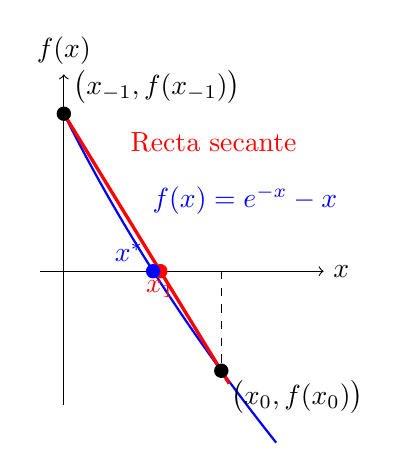
\begin{tikzpicture}[scale=2]

  % Ejes
  \draw[->]
    (-0.15,0) -- (1.65,0)
    node[right] {$x$};

  \draw[->]
    (0,-0.85) -- (0,1.25)
    node[above] {$f(x)$};

  % Curva f(x)=e^{-x}-x
  \draw[
    domain=0:1.35,
    samples=150,
    smooth,
    variable=\x,
    thick,
    blue
  ]
  plot ({\x},{exp(-\x)-\x});

  % Línea secante entre los puntos iniciales
  \draw[
    domain=0:1.05,
    samples=2,
    variable=\x,
    very thick,
    red
  ]
  plot ({\x},{1-1.63212056*\x});

  % Líneas verticales
  \draw[dashed]
    (1,0) -- (1,{exp(-1)-1});

  % Puntos sobre la función
  \filldraw[black]
    (0,1) circle (1.2pt)
    node[above right]
    {\(\bigl(x_{-1},f(x_{-1})\bigr)\)};

  \filldraw[black]
    (1,{exp(-1)-1}) circle (1.2pt)
    node[below right]
    {\(\bigl(x_0,f(x_0)\bigr)\)};

  % Intersección de la secante
  \filldraw[red]
    (0.61269984,0) circle (1.2pt)
    node[below]
    {\(x_1\)};

  % Raíz verdadera
  \filldraw[blue]
    (0.56714329,0) circle (1.2pt)
    node[above left]
    {\(x^*\)};

  % Etiquetas
  \node[blue] at (1.15,0.45)
    {\(f(x)=e^{-x}-x\)};

  \node[red] at (0.95,0.82)
    {Recta secante};

\end{tikzpicture}

\vspace{0.4em}

La recta que une
\(\bigl(x_{-1},f(x_{-1})\bigr)\) y
\(\bigl(x_0,f(x_0)\bigr)\)
cruza el eje \(x\) en la nueva aproximación \(x_1\).

\end{frame}


%========================================================
% SECANTE CONTRA FALSA POSICIÓN
%========================================================

\begin{frame}{Comparación: Secante y Falsa Posición}
\textbf{Similitudes:}
\begin{itemize}
  \item Ambas utilizan dos puntos de la función.
  \item Ambas aproximan la raíz mediante una recta secante.
  \item Ambas emplean la expresión:
  \(
  x_r
  =
  x_b
  -
  f(x_b)
  \frac{x_b-x_a}{f(x_b)-f(x_a)}.
  \)
\end{itemize}
\textbf{Diferencia principal:}
\begin{itemize}
  \item \textbf{Falsa posición:}
  conserva un intervalo que encierra la raíz. El nuevo valor reemplaza
  al extremo que tiene su mismo signo.
  \item \textbf{Secante:}
  utiliza siempre las dos aproximaciones más recientes, sin conservar
  necesariamente un intervalo que encierre la raíz.
\end{itemize}
Si \(f\) es continua y falsa posición inicia con un cambio de signo,
conserva el encerramiento de la raíz. La secante puede ser más rápida,
pero también puede divergir.

\end{frame}


%========================================================
% EJEMPLO DE COMPARACIÓN
%========================================================

\begin{frame}{Ejemplo: Comparación de Métodos}
\textbf{Función:}
\[
f(x)=\ln x.
\]
\textbf{Valores iniciales:}
\(
x_{-1}=0.5,
\qquad
x_0=5.
\)
\begin{columns}[T]
\begin{column}{0.48\textwidth}
\textbf{Falsa posición:}
\begin{itemize}
  \item \(x_{r,1}=1.854635\)
  \item \(x_{r,2}=1.216308\)
  \item \(x_{r,3}=1.058521\)
  \item \(x_{r,4}=1.016169\)
  \item \(x_r\longrightarrow1\)
\end{itemize}
\end{column}
\begin{column}{0.48\textwidth}
\textbf{Secante:}
\begin{itemize}
  \item \(x_1=1.854635\)
  \item \(x_2=-0.104381\)
  \item \(\ln(x_2)\) no está definido
        en los números reales.
\end{itemize}

\textcolor{red}{El método falla en el dominio real.}
\end{column}
\end{columns}
\textbf{Conclusión:}
Para este valor inicial, falsa posición conserva el intervalo
\([0.5,5]\), mientras que la secante genera una aproximación fuera
del dominio de \(\ln x\).

\end{frame}


%========================================================
% ALGORITMO DEL MÉTODO DE LA SECANTE
%========================================================

\begin{frame}[fragile]{Algoritmo en Python: Método de la Secante}

\begin{lstlisting}[
  style=mypython,
  basicstyle=\scriptsize\ttfamily,
  frame=single
]
def secante(f, xa, xb, es=1e-5,ftol=1e-10, imax=100):
    ea = float("inf")
    for i in range(imax):
        fa = f(xa)
        fb = f(xb)
        denominador = fb - fa
        if abs(denominador) < 1e-14:
            raise ZeroDivisionError(
                "Pendiente secante casi nula"
            )
        xc = xb - fb * (xb - xa) / denominador
        ea = abs(xc - xb) / max(
            abs(xc), 1e-12
        ) * 100
        if ea < es and abs(f(xc)) < ftol:
            return xc, i + 1, ea
        xa, xb = xb, xc
    return xc, imax, ea
\end{lstlisting}

\end{frame}


%========================================================
% VALIDACIONES DEL ALGORITMO
%========================================================

\begin{frame}{Validaciones del Algoritmo de la Secante}

\textbf{El algoritmo incluye:}

\begin{itemize}
  \item Verificación de pendiente secante cercana a cero:
  \[
  |f(x_i)-f(x_{i-1})|<\delta.
  \]

  \item Criterio de terminación por error relativo aproximado:
  \[
  \varepsilon_a
  =
  \left|
  \frac{x_{i+1}-x_i}{x_{i+1}}
  \right|100\%.
  \]

  \item Verificación del residuo:
  \[
  |f(x_{i+1})|<\varepsilon_f.
  \]

  \item Número máximo de iteraciones.

  \item Retorno de la raíz aproximada, el número de iteraciones
        y el último error aproximado.
\end{itemize}

\end{frame}


%========================================================
% MÉTODO DE LA SECANTE MODIFICADA
%========================================================

\begin{frame}{Método de la Secante Modificada}

\textbf{Enfoque alternativo:}
Aproximar la derivada utilizando una perturbación fraccionaria:
\(
h_i=d\,x_i.
\)
Si \(x_i\neq0\):
\[
f'(x_i)
\approx
\frac{f(x_i+h_i)-f(x_i)}{h_i}
=
\frac{f(x_i+d x_i)-f(x_i)}{d x_i}.
\]
Sustituyendo esta aproximación en Newton-Raphson:
\[
\boxed{
x_{i+1}
=
x_i
-
\frac{f(x_i)d x_i}
{f(x_i+d x_i)-f(x_i)}
}
\]
\begin{itemize}
  \item Solo requiere un valor inicial \(x_0\).
  \item No requiere una derivada analítica.
  \item Utiliza una evaluación adicional de la función.
  \item Si \(x_i=0\), debe emplearse una perturbación absoluta.
\end{itemize}

\end{frame}


%========================================================
% ALGORITMO DE LA SECANTE MODIFICADA
%========================================================

\begin{frame}[fragile]{Algoritmo en Python: Secante Modificada}
\begin{lstlisting}[
  style=mypython,
  basicstyle=\scriptsize\ttfamily,
  frame=single
]
def secante_modificada(f, x0, d=0.01, es=1e-5, ftol=1e-10, imax=100):
    for i in range(imax):
        fx = f(x0)
        if abs(x0) > 1e-12:
            h = d * x0
        else:
            h = d
        diferencia = f(x0 + h) - fx
        if abs(diferencia) < 1e-14:
            raise ZeroDivisionError(
                "Diferencia funcional casi nula"
            )
        x1 = x0 - fx * h / diferencia
        ea = abs(x1 - x0) / max(
            abs(x1), 1e-12
        ) * 100
        if ea < es and abs(f(x1)) < ftol:
            return x1, i + 1, ea
        x0 = x1
    return x1, imax, ea
\end{lstlisting}

\end{frame}


%========================================================
% ELECCIÓN DE LA PERTURBACIÓN
%========================================================

\begin{frame}{Elección de la Perturbación \(d\)}

En la secante modificada, el valor de \(d\) determina el tamaño
de la perturbación:
\(
h_i=d\,x_i.
\)
\begin{itemize}
  \item Si \(d\) es demasiado grande, la aproximación de la
        derivada puede ser poco precisa.
  \item Si \(d\) es demasiado pequeño, puede presentarse
        cancelación numérica en:
  \[
  f(x_i+h_i)-f(x_i).
  \]
  \item Si \(x_i\) está cerca de cero, \(h_i=d x_i\) puede ser
        demasiado pequeño o nulo.
  \item Una estrategia práctica es utilizar:
  \[
  h_i=
  \begin{cases}
  d x_i, & |x_i|>\delta,\\
  d,     & |x_i|\leq\delta.
  \end{cases}
  \]
\end{itemize}
\textbf{Conclusión:}
La elección de \(d\) debe equilibrar precisión y estabilidad numérica.
\end{frame}


%========================================================
% EJEMPLO DE LA SECANTE MODIFICADA
%========================================================

\begin{frame}{Ejemplo 8: Método de la Secante Modificada}

\textbf{Función y parámetros:}

\[
f(x)=e^{-x}-x,
\qquad
x^*\approx0.56714329,
\qquad
d=0.01,
\qquad
x_0=1.
\]

\centering
\small

\begin{tabular}{|c|c|c|}
\hline
\textbf{Iteración} &
\(\boldsymbol{x_i}\) &
\(\boldsymbol{\varepsilon_{t,i}(\%)}\) \\ \hline
0 & 1.000000000 & 76.3221 \\ 
1 & 0.537262666 & 5.2686 \\ 
2 & 0.567009685 & 0.02356 \\ 
3 & 0.567143424 & \(2.36\times10^{-5}\) \\ 
4 & 0.567143290 & \(2.42\times10^{-8}\) \\ \hline
\end{tabular}

\vspace{0.7em}

\raggedright

\textbf{Observación:}
El método converge rápidamente sin utilizar una derivada analítica.
Sin embargo, su comportamiento depende de la selección de \(d\).

\end{frame}


%========================================================
% CIRCUITO RLC: FORMULACIÓN DEL MODELO
%========================================================

\subsection{Aplicación: Circuito RLC}

\begin{frame}{Dise\~no de un Circuito El\'ectrico}

\textbf{Contexto:}
Estudio de la respuesta transitoria de un circuito RLC en serie
sin fuente externa.
\begin{itemize}
  \item El capacitor posee inicialmente una carga \(q_0\).
  \item La energ\'ia almacenada puede producir oscilaciones amortiguadas.
  \item La resistencia \(R\) disipa energ\'ia y controla el amortiguamiento.
\end{itemize}
\textbf{Relaciones b\'asicas:}
\[
i(t)=\frac{dq}{dt},
\qquad
V_R=Ri,
\qquad
V_L=L\frac{di}{dt},
\qquad
V_C=\frac{q}{C}.
\]
Aplicando la segunda ley de Kirchhoff:
\[
V_L+V_R+V_C=0.
\]
Por tanto:
\[
\boxed{
L\frac{d^2q}{dt^2}
+
R\frac{dq}{dt}
+
\frac{q}{C}
=0
}
\]
\end{frame}


%========================================================
% SOLUCIÓN DEL MODELO
%========================================================

\begin{frame}{Dise\~no de un Circuito El\'ectrico (2/5)}

Para el caso subamortiguado, la soluci\'on general es:

\[
q(t)
=
e^{-\alpha t}
\left(
A\cos(\omega_d t)
+
B\sin(\omega_d t)
\right),
\]
\[
\alpha=\frac{R}{2L},
\qquad
\omega_d
=
\sqrt{
\frac{1}{LC}
-
\frac{R^2}{4L^2}
}.
\]
\textbf{Condiciones iniciales:}
\[
q(0)=q_0=CV_0,
\qquad
i(0)=q'(0)=0.
\]
Estas condiciones producen:
\[
A=q_0,
\qquad
B=\frac{\alpha q_0}{\omega_d}.
\]

\end{frame}


%========================================================
% SOLUCIÓN PARTICULAR Y DATOS
%========================================================

\begin{frame}{Dise\~no de un Circuito El\'ectrico (3/5)}

La respuesta normalizada de la carga es:

\[
\frac{q(t)}{q_0}
=
e^{-\alpha t}
\left[
\cos(\omega_d t)
+
\frac{\alpha}{\omega_d}
\sin(\omega_d t)
\right].
\]

\textbf{Datos del dise\~no:}\(
L=5\ \text{H},
\qquad
C=10^{-4}\ \text{F},
\qquad
t=0.05\ \text{s}.
\)

Se desea que, en el instante \(t=0.05\ \text{s}\),

\(
\frac{q(0.05)}{q_0}=0.01.
\)

Con los valores dados:

\(
\alpha=\frac{R}{10},
\)

\(
\omega_d
=
\sqrt{
2000-0.01R^2
}.
\)

\end{frame}


%========================================================
% ECUACIÓN NO LINEAL
%========================================================

\begin{frame}{Dise\~no de un Circuito El\'ectrico (4/5)}
Sustituyendo \(t=0.05\) en la respuesta normalizada:
\[
\begin{aligned}
\phi(R)
={}&e^{-0.005R}
\left[
\cos\left(
0.05\sqrt{2000-0.01R^2}
\right)\right.\\
&\left.
+\frac{R/10}{\sqrt{2000-0.01R^2}}
\sin\left(
0.05\sqrt{2000-0.01R^2}
\right)
\right]
-0.01.
\end{aligned}
\]
La resistencia buscada satisface:
\(
\boxed{\phi(R)=0}
\)
 una respuesta subamortiguada: \(2000-0.01R^2>0.\)
Por tanto:
\(
0<R<447.2136\ \Omega.
\)

Se selecciona el intervalo inicial:\([0,400].\)
Además:\(
\phi(0)\approx-0.62727,
\qquad
\phi(400)\approx0.29088.
\)

Como existe cambio de signo, puede aplicarse bisecci\'on.

\end{frame}

%========================================================
% IMPLEMENTACIÓN NUMÉRICA
%========================================================

\begin{frame}{Dise\~no de un Circuito El\'ectrico (5/5)}

\textbf{Implementaci\'on num\'erica:}

\begin{itemize}
  \item M\'etodo empleado: bisecci\'on.
  \item Intervalo inicial: \([0,400]\).
  \item N\'umero de iteraciones: \(21\).
  \item Resistencia aproximada:
  \(
  \boxed{
  R\approx197.9285\ \Omega
  }
  \)
  \item Error relativo aproximado:
  \[
  \varepsilon_a<10^{-4}\%.
  \]
\end{itemize}

\textbf{Verificaci\'on:}
\[
\frac{q(0.05)}{q_0}
\approx0.01.
\]
La resistencia calculada permite que la carga sea aproximadamente
el \(1\%\) de su valor inicial en el instante \(t=0.05\ \text{s}\).

\end{frame}


%========================================================
% CONCLUSIONES
%========================================================

\begin{frame}{Dise\~no de un Circuito El\'ectrico: Conclusiones}
\begin{itemize}
  \item El modelo diferencial describe la respuesta transitoria
        del circuito RLC en serie.

  \item La resistencia determina el amortiguamiento y la velocidad
        con la que se disipa la energ\'ia almacenada.

  \item El m\'etodo de bisecci\'on permite calcular \(R\) sin
        derivar la ecuaci\'on trascendental.

  \item Con \(R\approx197.9285\ \Omega\), se obtiene:
  \(
  \frac{q(0.05)}{q_0}\approx0.01.
  \)

  \item Esta condici\'on se cumple en el instante especificado,
        pero no implica necesariamente que la carga permanezca
        por debajo del \(1\%\) para todo \(t>0.05\ \text{s}\).
\end{itemize}

\textbf{Aplicaciones:}
Dise\~no de filtros, circuitos de temporizaci\'on, sistemas de
telecomunicaciones y control de respuestas transitorias.

\end{frame}












% ==========================
% Diapositiva 1 – Título de sección
% ==========================
\subsection{Raíces de Polinomios}

\begin{frame}{Raíces de polinomios}
  \begin{itemize}
    \item En este tema estudiaremos métodos numéricos para encontrar las raíces de ecuaciones polinomiales.
    \item Polinomio de grado \(n\):
    \[
      f_n(x) = a_0 + a_1 x + a_2 x^2 + \dots + a_n x^n,
    \]
    donde los coeficientes \(a_i\) son constantes (reales en nuestra discusión).
    \item Las raíces del polinomio pueden ser reales y/o complejas.
  \end{itemize}
\end{frame}

% ==========================
% Diapositiva 2 – Propiedades básicas de las raíces
% ==========================
\begin{frame}{Propiedades de las raíces de un polinomio}
  \begin{itemize}
    \item Para una ecuación de grado \(n\), existen \(n\) raíces (reales o complejas), contadas con multiplicidad.
    \item Si \(n\) es impar, siempre hay al menos una raíz real.
    \item Si existen raíces complejas, aparecen en pares conjugados:
    \[
      \lambda \pm \mu i,
    \]
    con \(\lambda, \mu \in \mathbb{R}\) e \(i = \sqrt{-1}\).
  \end{itemize}
\end{frame}

% ==========================
% Diapositiva 3 – Polinomios en ciencia e ingeniería
% ==========================
\begin{frame}{Polinomios en la ciencia y la ingeniería}
  \begin{itemize}
    \item Los polinomios se usan ampliamente en:
    \begin{itemize}
      \item Ajuste de curvas (interpolación y aproximación).
      \item Modelado y caracterización de sistemas dinámicos.
      \item Análisis de sistemas lineales (mecánicos, estructurales, eléctricos, etc.).
    \end{itemize}
    \item En sistemas dinámicos lineales, los polinomios aparecen en las \textbf{ecuaciones características}.
    \item Sus raíces (eigenvalores) están directamente relacionadas con la \textbf{respuesta temporal} del sistema.
  \end{itemize}
\end{frame}

% ==========================
% Diapositiva 4 – Modelo de sistema de segundo orden
% ==========================
\begin{frame}{Sistema físico de segundo orden}
  Consideremos un sistema físico modelado por la siguiente EDO lineal:
  \[
    a_2 \frac{d^2 y}{dt^2} + a_1 \frac{dy}{dt} + a_0 y = F(t),
  \]
  donde:
  \begin{itemize}
    \item \(y(t)\): variable dependiente (respuesta del sistema).
    \item \(t\): variable independiente (tiempo).
    \item \(a_0, a_1, a_2\): coeficientes constantes del sistema.
    \item \(F(t)\): función de fuerza externa (término no homogéneo).
  \end{itemize}
\end{frame}

% ==========================
% Diapositiva 5 – Transformación a sistema de primer orden
% ==========================
\begin{frame}{Transformación a sistema de primer orden}
  Definimos una nueva variable:
  \[
    z = \frac{dy}{dt}.
  \]
  Entonces, el sistema de segundo orden puede escribirse como:
  \[
    \frac{dz}{dt} = \frac{1}{a_2}\big(F(t) - a_1 z - a_0 y\big),
  \]
  \[
    \frac{dy}{dt} = z.
  \]
  \begin{itemize}
    \item En general, una EDO lineal de orden \(n\) puede transformarse en un sistema de \(n\) EDO de primer orden.
    \item Esta forma es útil para análisis numérico e implementación computacional.
  \end{itemize}
\end{frame}

% ==========================
% Diapositiva 6 – Ecuación homogénea y solución general
% ==========================
\begin{frame}{Ecuación homogénea de segundo orden}
  Para estudiar la dinámica intrínseca del sistema, consideramos la ecuación homogénea:
  \[
    a_2 \frac{d^2 y}{dt^2} + a_1 \frac{dy}{dt} + a_0 y = 0.
  \]
  Buscamos soluciones de la forma:
  \[
    y(t) = e^{rt}.
  \]
  Sustituyendo en la ecuación homogénea se obtiene:
  \[
    a_2 r^2 e^{rt} + a_1 r e^{rt} + a_0 e^{rt} = 0
    \quad \Rightarrow \quad
    a_2 r^2 + a_1 r + a_0 = 0.
  \]
  \begin{itemize}
    \item Esta ecuación se llama \textbf{ecuación característica}.
    \item Sus raíces \(r\) son los \textbf{eigenvalores} del sistema.
  \end{itemize}
\end{frame}

% ==========================
% Diapositiva 7 – Eigenvalores y ecuación característica
% ==========================
\begin{frame}{Ecuación característica y eigenvalores}
  \[
    a_2 r^2 + a_1 r + a_0 = 0.
  \]
  Usando la fórmula cuadrática:
  \[
    r_{1,2} = \frac{-a_1 \pm \sqrt{a_1^2 - 4 a_2 a_0}}{2a_2}.
  \]
  \begin{itemize}
    \item Las raíces \(r_1, r_2\) determinan la forma de la solución general.
    \item Cada tipo de raíz se asocia con un tipo de \textbf{amortiguamiento} en la respuesta del sistema:
    \begin{itemize}
      \item Sobreamortiguado.
      \item Críticamente amortiguado.
      \item Subamortiguado.
    \end{itemize}
  \end{itemize}
\end{frame}

% ==========================
% Diapositiva 8 – Caso sobreamortiguado
% ==========================
\begin{frame}{Caso sobreamortiguado}
  Si el discriminante es positivo:
  \[
    a_1^2 - 4 a_2 a_0 > 0,
  \]
  entonces las raíces son reales y distintas:
  \[
    r_1, r_2 \in \mathbb{R}, \quad r_1 \neq r_2.
  \]
  La solución general es:
  \[
    y(t) = c_1 e^{r_1 t} + c_2 e^{r_2 t},
  \]
  donde \(c_1\) y \(c_2\) son constantes determinadas por las condiciones iniciales.
  \begin{itemize}
    \item Este caso se denomina \textbf{sobreamortiguado}.
    \item El sistema no oscila; la respuesta decae de forma exponencial (en general, lenta y sin oscilaciones).
  \end{itemize}
\end{frame}

% ==========================
% Diapositiva 9 – Amortiguamiento crítico
% ==========================
\begin{frame}{Caso de amortiguamiento crítico}
  Si el discriminante es cero:
  \[
    a_1^2 - 4 a_2 a_0 = 0,
  \]
  entonces hay una raíz real doble:
  \[
    r_1 = r_2 = \lambda.
  \]
  La solución general toma la forma:
  \[
    y(t) = (c_1 + c_2 t) e^{\lambda t}.
  \]
  \begin{itemize}
    \item Este caso se llama \textbf{amortiguamiento crítico}.
    \item El sistema retorna al equilibrio sin oscilar y, en cierto sentido, lo hace tan rápido como es posible sin llegar a oscilar.
  \end{itemize}
\end{frame}

% ==========================
% Diapositiva 10 – Caso subamortiguado (raíces complejas)
% ==========================
\begin{frame}{Caso subamortiguado: raíces complejas}
  Si el discriminante es negativo:
  \[
    a_1^2 - 4 a_2 a_0 < 0,
  \]
  las raíces son complejas conjugadas:
  \[
    r_{1,2} = \lambda \pm \mu i.
  \]
  La solución general puede escribirse inicialmente como:
  \[
    y(t) = c_1 e^{(\lambda + \mu i)t} + c_2 e^{(\lambda - \mu i)t}.
  \]
  Usando la fórmula de Euler:
  \[
    e^{\mu i t} = \cos(\mu t) + i \sin(\mu t),
  \]
  se obtiene una forma real equivalente:
  \[
    y(t) = c_1 e^{\lambda t} \cos(\mu t) + c_2 e^{\lambda t} \sin(\mu t).
  \]
  \begin{itemize}
    \item Este caso se denomina \textbf{subamortiguado}.
    \item La respuesta es oscilatoria con una envolvente exponencial.
  \end{itemize}
\end{frame}

% ==========================
% Diapositiva 11 – Interpretación física de los eigenvalores
% ==========================
\begin{frame}{Interpretación física de los eigenvalores}
  \begin{itemize}
    \item \textbf{Parte real} de \(r\):
    \begin{itemize}
      \item Si \(\Re(r) < 0\): la respuesta decae en el tiempo (estable).
      \item Si \(\Re(r) > 0\): la respuesta crece en el tiempo (inestable).
    \end{itemize}
    \item \textbf{Parte imaginaria} de \(r\):
    \begin{itemize}
      \item Indica la presencia de términos senoidales \(\cos(\mu t)\), \(\sin(\mu t)\).
      \item El sistema presenta oscilaciones con frecuencia \(\mu\).
    \end{itemize}
    \item Cuando el eigenvalor tiene parte real e imaginaria:
    \begin{itemize}
      \item La respuesta combina decaimiento (o crecimiento) exponencial y oscilaciones.
    \end{itemize}
  \end{itemize}
  \vspace{0.3cm}
  \begin{block}{Idea clave}
    El análisis de las raíces de la ecuación característica permite entender, diseñar y controlar el comportamiento dinámico de sistemas físicos.
  \end{block}
\end{frame}


% ==========================
% Diapositiva: Cálculos con polinomios
% ==========================
\begin{frame}{Cálculos con polinomios}
  \textbf{Objetivo:} realizar operaciones básicas necesarias para los métodos de búsqueda de raíces.

  \begin{block}{Evaluación eficiente: método de Horner}
    Polinomio de grado \(n\):
    \[
      f(x) = a_0 + a_1 x + a_2 x^2 + \dots + a_n x^n.
    \]
    \begin{itemize}
      \item Forma directa: requiere \(\dfrac{n(n+1)}{2}\) multiplicaciones.
      \item \textbf{Forma anidada (Horner)}:
      \[
        f(x) = (\cdots((a_n x + a_{n-1})x + a_{n-2})x + \dots + a_0,
      \]
      usa solo \(n\) multiplicaciones y \(n\) sumas.
      \item Menos operaciones \(\Rightarrow\) menos error de redondeo.
    \end{itemize}
  \end{block}

  \begin{block}{Derivada con Horner modificado}
    Con una ligera modificación del algoritmo de Horner se puede obtener, en el mismo ciclo,
    \(f(x)\) y \(f'(x)\), lo cual es clave, por ejemplo, en el método de Newton-Raphson.
  \end{block}
\end{frame}

% ==========================
% Diapositiva: Deflación polinomial
% ==========================
\begin{frame}{Deflación polinomial}
  \begin{itemize}
    \item Si se conoce una raíz aproximada \(t\) de un polinomio \(f(x)\), es útil \textbf{“sacarla”} del polinomio.
    \item Se divide \(f(x)\) entre el factor \((x - t)\) (o un factor cuadrático), reduciendo el grado.
    \item Esto evita volver a encontrar la misma raíz y simplifica el problema.
  \end{itemize}

  \begin{block}{Idea básica}
    \begin{itemize}
      \item Representar el polinomio por sus coeficientes.
      \item Aplicar una forma de \textbf{división sintética}:
        \[
          f(x) = (x - t)\,q(x) + r,
        \]
        donde \(q(x)\) es el polinomio deflactado y \(r\) el residuo.
      \item Si \(t\) es raíz exacta, \(r = 0\).
    \end{itemize}
  \end{block}

  \begin{itemize}
    \item En la práctica numérica: la deflación es sensible a errores de redondeo.
    \item A veces se “pulen” las raíces usando de nuevo el polinomio original.
  \end{itemize}
\end{frame}

% =========================================
% Diapositiva 1 – Idea del método de Müller
% =========================================
\begin{frame}{Método de Müller}
  \begin{itemize}
    \item El método de la secante aproxima la raíz trazando una \textbf{recta}
    que pasa por dos puntos \((x_0, f(x_0))\) y \((x_1, f(x_1))\), y extendiéndola
    hasta cortar el eje \(x\).
    \item El \textbf{método de Müller} generaliza esta idea:
    \begin{itemize}
      \item En lugar de una recta, ajusta una \textbf{parábola} que pasa por
            tres puntos: \((x_0, f(x_0))\), \((x_1, f(x_1))\), \((x_2, f(x_2))\).
      \item Luego usa la \textbf{fórmula cuadrática} para encontrar la intersección
            de la parábola con el eje \(x\).
    \end{itemize}
    \item Ventaja importante:
    \begin{itemize}
      \item Puede converger a \textbf{raíces reales y complejas}.
    \end{itemize}
  \end{itemize}
\end{frame}

% ==================================================
% Diapositiva 2 – Parábola interpolante y coeficientes
% ==================================================
\begin{frame}{Parábola interpolante en el método de Müller}
  Se plantea una parábola de la forma
  \[
    f_2(x) = a(x - x_2)^2 + b(x - x_2) + c
  \]
  que pasa por:
  \[
    (x_0, f(x_0)), \quad (x_1, f(x_1)), \quad (x_2, f(x_2)).
  \]

  \begin{itemize}
    \item Al evaluar en \(x = x_2\), se tiene inmediatamente:
      \[
        c = f(x_2).
      \]
    \item Con \(x_0\) y \(x_1\) se obtienen dos ecuaciones adicionales que
          permiten calcular \(a\) y \(b\).
  \end{itemize}

  Para simplificar la notación se introducen las diferencias:
  \[
    h_0 = x_1 - x_0, \quad h_1 = x_2 - x_1,
  \]
  \[
    d_0 = \frac{f(x_1) - f(x_0)}{x_1 - x_0}, \quad
    d_1 = \frac{f(x_2) - f(x_1)}{x_2 - x_1}.
  \]
\end{frame}

% ==================================================
% Diapositiva 3 – Fórmulas para a, b y c
% ==================================================
\begin{frame}{Cálculo de los coeficientes a, b y c}
  A partir de las ecuaciones que resultan de imponer que la parábola pase por
  los tres puntos, se obtienen:

  \[
    a = \frac{d_1 - d_0}{h_1 + h_0},
  \]
  \[
    b = a\,h_1 + d_1,
  \]
  \[
    c = f(x_2).
  \]

  \begin{itemize}
    \item Estos coeficientes describen la parábola interpolante en torno a \(x_2\).
    \item El siguiente paso es aplicar la \textbf{fórmula cuadrática}
          sobre esta parábola para estimar la raíz.
  \end{itemize}
\end{frame}

% ==================================================
% Diapositiva 4 – Cálculo de la nueva aproximación
% ==================================================
\begin{frame}{Cálculo de la nueva aproximación \(x_3\)}
  La parábola se escribe como
  \[
    f_2(x) = a(x - x_2)^2 + b(x - x_2) + c = 0.
  \]

  Aplicando la fórmula cuadrática en la variable \((x - x_2)\):

  \[
    x_3 = x_2 + \frac{-2c}{b \pm \sqrt{b^2 - 4ac}}.
  \]

  \begin{itemize}
    \item El signo del denominador se elige para \textbf{maximizar}
          \(|b \pm \sqrt{b^2 - 4ac}|\), es decir, se escoge el signo que tenga
          la \textbf{misma} orientación que \(b\).
    \item Esta elección reduce el efecto del error de redondeo y suele
          dar una mejor aproximación.
  \end{itemize}

  El error relativo aproximado puede estimarse como:
  \[
    \varepsilon_a \approx \left|\frac{x_3 - x_2}{x_3}\right| \times 100\%.
  \]
\end{frame}

% ==================================================
% Diapositiva 5 – Estrategia iterativa
% ==================================================
\begin{frame}{Estrategia iterativa del método de Müller}
  Una vez obtenida la nueva aproximación \(x_3\), el proceso se repite.

  \begin{block}{Actualización de los puntos}
    Existen dos estrategias frecuentes:
    \begin{enumerate}
      \item \textbf{Sólo raíces reales:} se conservan los dos puntos
            anteriores más cercanos a \(x_3\) y se descarta el más lejano.
      \item \textbf{Raíces reales y complejas:} se usa una actualización
            secuencial:
            \[
              x_0 \leftarrow x_1, \quad
              x_1 \leftarrow x_2, \quad
              x_2 \leftarrow x_3.
            \]
    \end{enumerate}
  \end{block}

  \begin{itemize}
    \item El proceso continúa hasta que el error relativo \(\varepsilon_a\)
          sea menor que una tolerancia prefijada o se alcance un número
          máximo de iteraciones.
  \end{itemize}
\end{frame}

% ==================================================
% Diapositiva 6 – Pseudocódigo del método de Müller
% ==================================================
\begin{frame}[fragile]{Pseudocódigo del método de Müller}
  \begin{block}{Müller para raíces (posiblemente reales)}
\begin{verbatim}
Dado: xr (estimación inicial), h, eps, maxit
x2 = xr
x1 = xr + h*xr
x0 = xr - h*xr

REPETIR
  h0 = x1 - x0
  h1 = x2 - x1
  d0 = (f(x1) - f(x0)) / h0
  d1 = (f(x2) - f(x1)) / h1

  a = (d1 - d0) / (h1 + h0)
  b = a*h1 + d1
  c = f(x2)

  rad = sqrt(b*b - 4*a*c)
  si |b + rad| > |b - rad|
      den = b + rad
    si no
      den = b - rad
  fin si

  dxr = -2*c / den
  xr  = x2 + dxr

  comprobar criterio de paro con dxr
  actualizar x0, x1, x2 (por ejemplo: x0=x1, x1=x2, x2=xr)
HASTA converger o alcanzar maxit
\end{verbatim}
  \end{block}
\end{frame}

% ==================================================
% Diapositiva 7 – Ejemplo (esquema)
% ==================================================
\begin{frame}{Ejemplo: \(f(x) = x^3 - 13x - 12\)}
  \begin{itemize}
    \item Función:
      \[
        f(x) = x^3 - 13x - 12.
      \]
    \item Supongamos valores iniciales:
      \[
        x_0 = 4.5, \quad x_1 = 5.5, \quad x_2 = 5.
      \]
    \item Con estos valores:
      \begin{itemize}
        \item Se calculan \(h_0, h_1, d_0, d_1\).
        \item Luego \(a, b, c\) a partir de las fórmulas:
          \[
            a = \frac{d_1 - d_0}{h_1 + h_0}, \quad
            b = a\,h_1 + d_1, \quad
            c = f(x_2).
          \]
        \item Finalmente se obtiene \(x_3\) con:
          \[
            x_3 = x_2 + \frac{-2c}{b \pm \sqrt{b^2 - 4ac}}.
          \]
      \end{itemize}
    \item Repitiendo el proceso, el método converge rápidamente
          a la raíz real \(x_r = 4\).
  \end{itemize}
\end{frame}

% =========================================
% Diapositiva 1 – Idea general del método de Bairstow
% =========================================
\begin{frame}{Método de Bairstow}
  \begin{itemize}
    \item El método de Bairstow es un procedimiento iterativo para encontrar
          \textbf{todas} las raíces (reales y complejas) de un polinomio con coeficientes reales.
    \item Se basa en factorizar el polinomio original \(f_n(x)\) como:
      \[
        f_n(x) \approx (x^2 - r x - s)\, q_{n-2}(x) + R(x),
      \]
      donde:
      \begin{itemize}
        \item \(x^2 - r x - s\) es un \textbf{factor cuadrático} buscado.
        \item \(q_{n-2}(x)\) es el cociente de grado \(n-2\).
        \item \(R(x)\) es el residuo (de grado \(\leq 1\)).
      \end{itemize}
    \item Objetivo:
      \begin{itemize}
        \item Ajustar iterativamente \(r\) y \(s\) hasta que el residuo sea cero
              \(\Rightarrow\) el factor cuadrático es exacto.
        \item Las dos raíces (reales o complejas) se obtienen luego con la fórmula cuadrática.
      \end{itemize}
  \end{itemize}
\end{frame}

% =========================================
% Diapositiva 2 – División entre un factor cuadrático
% =========================================
\begin{frame}{División entre el factor cuadrático \(x^2 - r x - s\)}
  Sea
  \[
    f_n(x) = a_0 + a_1 x + a_2 x^2 + \dots + a_n x^n,
  \]
  un polinomio de grado \(n\).

  \begin{itemize}
    \item Lo dividimos entre \(x^2 - r x - s\) para obtener:
      \[
        f_n(x) = (x^2 - r x - s)\, q_{n-2}(x) + R(x),
      \]
      donde:
      \[
        q_{n-2}(x) = b_2 + b_3 x + \dots + b_n x^{n-2},
      \]
      \[
        R(x) = b_1 (x - r) + b_0.
      \]
    \item Los coeficientes \(b_i\) se calculan mediante las \textbf{relaciones de recurrencia}:
      \[
        b_n = a_n,
      \]
      \[
        b_{n-1} = a_{n-1} + r b_n,
      \]
      \[
        b_i = a_i + r b_{i+1} + s b_{i+2}, \quad \text{para } i = n-2,\dots,0.
      \]
    \item Si el factor cuadrático es exacto, el residuo se anula: \(b_0 = 0\) y \(b_1 = 0\).
  \end{itemize}
\end{frame}

% =========================================
% Diapositiva 3 – Condición de residuo nulo y corrección de r, s
% =========================================
\begin{frame}{Condición de residuo nulo y corrección de \(r\) y \(s\)}
  \begin{itemize}
    \item Para que \(x^2 - r x - s\) sea un divisor exacto de \(f_n(x)\),
          se requiere:
      \[
        b_0(r,s) = 0, \quad b_1(r,s) = 0.
      \]
    \item En general, con valores iniciales \((r,s)\), estos residuos no son cero.
    \item Se busca mejorar \((r,s)\) con incrementos \(\Delta r\) y \(\Delta s\)
          usando una \textbf{aproximación tipo Newton-Raphson} en dos variables:
      \[
        b_1(r+\Delta r,s+\Delta s) \approx b_1 +
          \frac{\partial b_1}{\partial r} \Delta r +
          \frac{\partial b_1}{\partial s} \Delta s,
      \]
      \[
        b_0(r+\Delta r,s+\Delta s) \approx b_0 +
          \frac{\partial b_0}{\partial r} \Delta r +
          \frac{\partial b_0}{\partial s} \Delta s.
      \]
    \item Igualando a cero estas expresiones, se obtiene un sistema lineal
          en \(\Delta r\) y \(\Delta s\).
  \end{itemize}
\end{frame}

% =========================================
% Diapositiva 4 – Cálculo de derivadas parciales por recurrencias c_i
% =========================================
\begin{frame}{Obtención de derivadas parciales: coeficientes \(c_i\)}
  \begin{itemize}
    \item Bairstow mostró que las derivadas parciales de \(b_0\) y \(b_1\)
          respecto a \(r\) y \(s\) se obtienen mediante una \textbf{segunda división sintética}
          sobre los \(b_i\).
    \item Se definen los coeficientes \(c_i\) con recurrencias análogas:
      \[
        c_n = b_n,
      \]
      \[
        c_{n-1} = b_{n-1} + r c_n,
      \]
      \[
        c_i = b_i + r c_{i+1} + s c_{i+2}, \quad \text{para } i = n-2,\dots,1.
      \]
    \item A partir de ellos:
      \[
        \frac{\partial b_0}{\partial r} = c_1, \quad
        \frac{\partial b_0}{\partial s} = c_2,
      \]
      \[
        \frac{\partial b_1}{\partial r} = c_2, \quad
        \frac{\partial b_1}{\partial s} = c_3.
      \]
  \end{itemize}
\end{frame}

% =========================================
% Diapositiva 5 – Sistema lineal para Δr y Δs
% =========================================
\begin{frame}{Sistema lineal para \(\Delta r\) y \(\Delta s\)}
  Usando las aproximaciones de Taylor y las derivadas parciales, se obtiene el sistema:
  \[
    c_2 \Delta r + c_3 \Delta s = -b_1,
  \]
  \[
    c_1 \Delta r + c_2 \Delta s = -b_0.
  \]

  \begin{itemize}
    \item Resolviendo este sistema, se obtienen las correcciones:
      \[
        \Delta r, \quad \Delta s.
      \]
    \item Los valores de \(r\) y \(s\) se actualizan como:
      \[
        r_{\text{nuevo}} = r + \Delta r, \quad
        s_{\text{nuevo}} = s + \Delta s.
      \]
    \item El proceso se repite hasta que los errores relativos:
      \[
        |e_{a,r}| = \left|\frac{\Delta r}{r}\right| 100\%, \quad
        |e_{a,s}| = \left|\frac{\Delta s}{s}\right| 100\%
      \]
      sean menores que una tolerancia \(e_s\) o se alcance un número máximo de iteraciones.
  \end{itemize}
\end{frame}

% =========================================
% Diapositiva 6 – Obtención de raíces y deflación
% =========================================
\begin{frame}{Obtención de raíces y deflación del polinomio}
  Una vez que se ha encontrado un factor cuadrático satisfactorio:
  \[
    x^2 - r x - s,
  \]
  las dos raíces asociadas se calculan mediante:
  \[
    x = \frac{r \pm \sqrt{r^2 + 4s}}{2}.
  \]

  \begin{itemize}
    \item Las raíces pueden ser:
      \begin{itemize}
        \item \textbf{Reales} si \(r^2 + 4s > 0\),
        \item \textbf{Complejas conjugadas} si \(r^2 + 4s < 0\).
      \end{itemize}
    \item A continuación, se \textbf{deflaciona} el polinomio original:
      \begin{itemize}
        \item Se reemplazan los coeficientes \(a_i\) por el cociente \(q_{n-2}(x)\)
              obtenido a partir de los \(b_i\).
        \item Se reduce el grado en 2 y se repite el proceso para encontrar
              el siguiente par de raíces.
      \end{itemize}
    \item Casos finales:
      \begin{itemize}
        \item Cociente de grado 2: se aplica directamente la fórmula cuadrática.
        \item Cociente de grado 1: la raíz restante es
          \[
            x = -\frac{a_0}{a_1}.
          \]
      \end{itemize}
  \end{itemize}
\end{frame}

% =========================================
% Diapositiva 7 – Comentarios y ventajas del método de Bairstow
% =========================================
\begin{frame}{Comentarios y ventajas del método de Bairstow}
  \begin{itemize}
    \item Permite encontrar \textbf{todas las raíces} de un polinomio con coeficientes reales,
          incluyendo \textbf{raíces complejas} (en pares conjugados).
    \item Utiliza sólo aritmética real (no requiere trabajar explícitamente
          con números complejos en el algoritmo principal).
    \item Se basa en:
      \begin{itemize}
        \item División sintética para calcular \(b_i\) (cociente y residuo).
        \item Una segunda división sintética para obtener \(c_i\) (derivadas parciales).
        \item Un esquema tipo Newton-Raphson en \((r,s)\).
      \end{itemize}
    \item Es especialmente adecuado para implementación en computadora:
      \begin{itemize}
        \item Estructura iterativa clara.
        \item Fórmulas de recurrencia sencillas.
      \end{itemize}
    \item Como todo método iterativo:
      \begin{itemize}
        \item Requiere buenos criterios de paro.
        \item Puede ser sensible a los valores iniciales \(r_0, s_0\) y al condicionamiento
              del polinomio.
      \end{itemize}
  \end{itemize}
\end{frame}


\end{document}

